\documentclass{book}
\usepackage{geometry}
 \geometry{
 a4paper,
 total={170mm,257mm},
 left=20mm,
 top=20mm,
 }
\usepackage[utf8]{inputenc}
\usepackage{hyperref}
\usepackage{braket}
\usepackage{amsmath}
\usepackage{amssymb}
\usepackage{amsthm}
\usepackage{mathtools}
\usepackage{amsfonts}
\usepackage{physics}
\usepackage{tikz-cd}
\usepackage{musicography}
\usepackage{enumerate}
\usepackage{xfrac}
\usepackage[parfill]{parskip}
\usepackage{subcaption}
\usepackage{float}
\usepackage{pgfplots}
\pgfplotsset{compat=1.12}
\usepgfplotslibrary{fillbetween}

\newcommand{\cm}{\mathbb{C}}
\newcommand{\re}{\mathbb{R}}
\newcommand{\dvg}{\nabla\cdot}
\newcommand{\crl}{\nabla\times}
\newcommand{\proj}[1]{\ensuremath{{\ket{#1}\bra{#1}}}}
\newcommand{\vect}{\text{Vect}}
\newcommand{\smooth}{C^{\infty}}
\newcommand{\dif}{\text{d}}

\makeatletter
\newcommand*\bigcdot{\mathpalette\bigcdot@{.8}}
\newcommand*\bigcdot@[2]{\mathbin{\vcenter{\hbox{\scalebox{#2}{$\m@th#1\bullet$}}}}}
\makeatother
\newlength{\arrow}
\settowidth{\arrow}{\scriptsize$1000$}
\newcommand*{\myrightarrow}[1]{\xrightarrow{\mathmakebox[\arrow]{#1}}}
\newcommand*{\TakeFourierOrnament}[1]{{%
\fontencoding{U}\fontfamily{futs}\selectfont\char#1}}
\newcommand*{\danger}{\TakeFourierOrnament{66}}
\setlength{\jot}{1.5mm}

\theoremstyle{definition}
\newtheorem{thm}{Theorem}[section] % the main one
\newtheorem{lemma}[thm]{Lemma}
\newtheorem{joke}{Joke}
% other statement types

% for specifying a name
\theoremstyle{plain} % just in case the style had changed
\newcommand{\thistheoremname}{}
\newtheorem{genericthm}[thm]{\thistheoremname}
\newenvironment{namedthm}[1]
  {\renewcommand{\thistheoremname}{#1}%
   \begin{genericthm}}
  {\end{genericthm}}
  
\newtheorem{defn}{Definition}
\newtheorem{prop}{Proposition}
\newtheorem{rmk}{Remark}
\newtheorem{conj}{Conjecture}
%\newtheorem{lemma}{Lemma}
\newtheorem{cor}{Corollary}
\newtheorem{problem}{Problem}




\begin{document}

\begin{center}
	\huge{Research notes}
	
	\small{All here is public}
\end{center}

\medskip
\hrule

\begin{enumerate}
    \item Cosmology
    \begin{itemize}
	\item Introduction
	\item General relativity
	\item $\Lambda$CDM
	\item Experiments: CMB and Weak Lensing
    \end{itemize}
    \item Tensions
    \begin{itemize}
	\item Introduction
	\item Estimators
	\item Metrics
    \end{itemize}
    \item Methodology
    \begin{itemize}
	\item MCMC
	\item Emulators
	\item Normalizing Flow
	\item Posterior Optimization
    \end{itemize}
    \item Results (and other things as they come up)
\end{enumerate}

\medskip
\hrule

%\section{Cosmology}
%\input{stats.tex}
\chapter{General Relativity and Cosmology}
\section{Motivation}
With Einstein's formulation of special relativity came a beautiful expansion of physics into the high energy and large scale regime. A postulate of special relativity was that light is a universal speed limit, and with this postulate a plethora of established physical theories became problematic. Fortunately for theories such as electromagnetism no incompatibilities were introduced. However, for gravity this was not the case. The gravitational field had no wave equation to establish a speed of propagation, meaning changes to the gravitational field were felt instantaneously globally. Attempts to reconcile this, such as using a retarded propagator or promoting the newtonian potential to a scalar field theory, proved incapable of correcting for relativity. Never-the-less, Newtonian gravity has stood the test of time to be accurate in the non-relativistic limit. Thus any theory of gravity should reduce to the Newtonian theory for speeds $v \ll c$.

The famous thought experiment of an Einstein elevator demonstrates a striking inconsistency within Newtonian gravity. Consider an observer freely falling in a spherical gravitational field. With nothing to look at, this person would not be able to determine they were in a gravitational field rather than just linearly accelerating. Now suppose this observer has point particles nearby, one to each side, one above, and one below (fig.). What the observer will see is the particles below and above them will move farther away because the gravitiational force scales as $1/r^2$. They will see the particles to the side of them moving towards them due to the spherical symmetry of the gravitational field. These fictitious forces are referred to as the tidal forces, as they also give rise to the seen twice per day on earth. This interesting thought experiment shows how freely falling reference frames are not inertial frames, the first inconsistency recognized by Einstein. 

In (year) Einstein published his first paper on special relativity. In special relativity, physical space is enhanced to a four dimensional space, typically denoted $\mathbb{M}^4$ or $\mathbb{R}^{3,1}$. Setting $c=1$ (which is done in the rest of this thesis), the metric is given by
\begin{equation}
    g = \text{diag}(-1,1,1,1)
\end{equation}
This space is typically called \textit{Minkowski space} (thus the notation $\mathbb{M}^4$). Distances under this metric are called the \textit{proper time} interval, denoted $\tau$.
\begin{equation}\label{eq:proper-time}
    -d\tau^2 = -dt^2 + dx^2 + dy^2 + dz^2
\end{equation}
Proper time represents the amount of time it that passes for an observer travelling on a path with 0 spatial displacement. Naturally, this quantity should be invariant even for an observer in a different reference frame. For such an observer, the time that elapses will be different from $\tau$, and will be accounted for by the spatial displacement as seen by equation~\ref{eq:proper-time}. The set of transformations that leave $\tau$ invariant are the Lorentz transformations.
\begin{figure}
    \centering
    \begin{tikzpicture}
        \draw (0,-2) -- (0,-0.5);
        \draw[dashed] (0,-0.5) -- (0,1.7);
        \draw (0,1.7) -- (0,2);
        \draw (-2,0) -- (2,0);
        \draw (0,2)  node[anchor=south] {$t$};
        \draw (2,0)  node[anchor=west] {$x$};
        \draw plot [smooth] coordinates {(-0.8,-1.5) (-0.3,-0.5) (0,0) (0.4,0.7) (-0.3,1.7) (-0.2,2.0)};
        \draw[fill=black] (-0.3,-0.5) circle (1pt);
        \draw[fill=black] (-0.3,1.7) circle (1pt);
        \draw[very thick] plot [smooth] coordinates {(-0.3,-0.5) (0,0) (0.4,0.7) (-0.3,1.7)};
        \draw (0.3,0.7) node [anchor=west] {$\Delta \tau$};
        \draw[fill=black] (0,-0.5) circle (1pt);
        \draw[fill=black] (0,1.7) circle (1pt);
        \draw (0,0.6) node [anchor=east] {$\Delta t$};
    \end{tikzpicture}
    \caption{Definition of proper time (bold line) vs. coordinate time (dashed line).}
\end{figure}
Lets suppose we have two observers, one is in an inertial frame with coordinates $x$ and the other is in a non-inertial frame with coordinates $x'$. These coordinates are related $x = x(x')$. In the inertial frame, the equations of motion are given by 
\begin{figure}
    \centering
    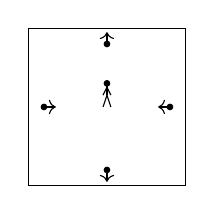
\begin{tikzpicture}
        \draw (-1,-1) -- (-1,1) -- (1,1) -- (1,-1) -- (-1,-1);
        \draw[fill=black] (0,0.3) circle (1pt);
        \draw (0,0.3) -- (0,0.15);
        \draw (0,0.15) -- (0.05,0);
        \draw (0,0.15) -- (-0.05,0);
        \draw (0,0.25) -- (0.05,0.15);
        \draw (0,0.25) -- (-0.05,0.15);
        \draw[fill=black] (-0.8,0) circle (1pt);
        \draw[fill=black] (0.8,0) circle (1pt);
        \draw[fill=black] (0,0.8) circle (1pt);
        \draw[fill=black] (0,-0.8) circle (1pt);
        \draw[->] (0,-0.8) -- (0,-0.95);
        \draw[->] (0,0.8) -- (0,0.95);
        \draw[->] (-0.8,0) -- (-0.65,0);
        \draw[->] (0.8,0) -- (0.65,0);
    \end{tikzpicture}
    \caption{Observer freely falling with particles experience tidal forces within the observers reference frame.}
\end{figure}
\begin{equation}
    \frac{d^2x^\mu}{d\tau^2} = 0
\end{equation} 
We can look at how this changes for the observer in a non-inertial frame.
\begin{equation}\label{eq:sr-curves}
    \frac{d^2x'^\lambda}{d\tau^2}+\underbrace{\frac{\partial x'^\lambda}{\partial x^\rho}\frac{\partial^2 x^\rho}{\partial x'^\mu \partial x'^\nu}}_{\equiv \Gamma_{\mu\nu}^\lambda} \frac{d x'^\mu}{d \tau} \frac{d x'^\nu}{d \tau} = 0
\end{equation}
Equation~\ref{eq:sr-curves} looks suspiciously like the geodesic equation from differential geometry. The exception is we have defined the `Chirstoffel symbol' here, which is not the most general form of the Christoffel symbols. This does give motivation for how to search for a compatible theory of gravity. However, this does provide a clear link between gravity and geometry. 
\section{Einstein's Field Equation}
Christoffel symbols take a very general form, where they signify the failure of partial derivatives to commute. This failure results from curvature of the space itself. As said in the previous section, special relativity promotes the classical $\mathbb{R}^3$ space to $\mathbb{M}^4$. However, we now need to allow curved space, not simply minkowski space. So lets take an arbitrary semi-Riemannian 4-manifold $M$. In very loose terms, a manifold is a locally euclidean space, which is a sufficient definition for this application.

Naturally, computing derivatives are difficult on curved surfaces. To start, derivatives give tangent vectors, thus taking the set of all possible tangent vectors of a curve at point $p\in M$ gives us the tangent space at $p$, denoted $T_pM$. The generalization of the derivative is called a \textit{connection}~\cite{baez_john_gauge_1994}, which tells one how to connect the tangent spaces at different points infinitessimally (figure~\ref{fig:parallel_transport}). Although beyond the scope of this thesis, it is worth noting that, due to the holonomy of curved surfaces, this will generally depend on the path taken.
\begin{figure}
    \centering
    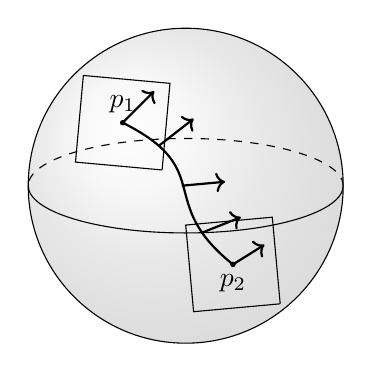
\begin{tikzpicture}
        \shade[ball color = gray!40, opacity = 0.2] (0,0) circle (2cm);
        \draw (0,0) circle (2cm);
        \draw (-2,0) arc (180:360:2 and 0.6);
        \draw[dashed] (2,0) arc (0:180:2 and 0.6);
        \fill[fill=black] (-0.8,0.8) circle (1pt);
        \draw (-0.8,0.8) node[anchor=south] {$p_1$};
        \fill[fill=black] (0.6,-1.0) circle (1pt);
        \draw (0.6,-1.0) node[anchor=north] {$p_2$};
        \draw (-0.8+0.5,0.8-0.6) -- (-0.8-0.6,0.8-0.5) -- (-0.8-0.5,0.8+0.6) -- (-0.8+0.6,0.8+0.5) -- (-0.8+0.5,0.8-0.6); %bottom right -- bottom left -- top left -- top right -- bottom right
        \draw (0.6+0.6,-1-0.5) -- (0.6-0.5,-1-0.6) -- (0.6-0.6,-1+0.5) -- (0.6+0.5,-1+0.6) -- (0.6+0.6,-1-0.5);
        \draw[thick] (-0.8,0.8) .. controls (0.4,0.2) and (-0.4,-0.2) .. (0.6,-1);
        \draw[->,thick] (-0.8,0.8) -- (-0.4,1.2);
        \draw[->,thick] (-0.35,0.5) -- (0.1,0.85);
        \draw[->,thick] (-0.05,0) -- (0.5,0.05);
        \draw[->,thick] (0.2,-0.6) -- (0.7,-0.4);
        \draw[->,thick] (0.6,-1) -- (1,-0.75);
    \end{tikzpicture}
    \caption{Example of parallel transport along a connection on a sphere. }
    \label{fig:parallel_transport}
\end{figure}
In general relativity, a very special connection is use called the \textit{Levi-Civita connection}, denoted $\nabla$, which is torsionless and metric preserving. More precisely, for all vector fields $u,v,w$ on $M$
\begin{equation}
    \begin{split}
        u g(v,w) =& g(\nabla_u v, w)+g(v,\nabla_uw) \,,\quad \text{(metric preserving)} \\
        [u,v] =& \nabla_u v - \nabla_v u \,,\quad \text{(torsion free)}
    \end{split}
\end{equation}

The only remaining geometric property for the Levi-Civita connection is curvature, which can be neatly described using the christoffel symbols defined by
\begin{equation}
    \nabla_\mu\partial_\nu = \Gamma^{\rho}_{\mu\nu}\partial_\rho\,.
\end{equation}
In this case, the partials here are refering to the basis of vector fields on $M$.Additionally this curvature has a special name as well, the \textit{Riemann curvature}, a type (3,1) tensor defined by
\begin{equation}
    R(u,v)w = (\nabla_u\nabla_v-\nabla_v\nabla_u - \nabla_{[u,v]})w
\end{equation}
or in coordinate form by
\begin{equation}
    R_{\mu\nu\rho}^\sigma  = \nabla_\mu \Gamma^\sigma_{\nu\rho} - \nabla_\nu\Gamma^{\sigma}_{\mu\rho}
\end{equation}
To emphasize the elegance of Einstein's equation, its convinient to note write the Riemann curvature as a matrix valued differential 2-form $\mathcal{R}$ and the christoffel symbols as a matrix valued differential 1-form $\mathcal{G}$ (differential forms are antisymmetric covariant tensors). With this notion, its easy to see the Bianchi identity for $\mathcal{R}$ with respect to the Levi-Civita connection is
\begin{equation}
    d_{\nabla}\mathcal{R} = \nabla_{[\tau}R^\sigma_{\mu\nu]\rho} = 0
\end{equation}
Where the brackets denote antisymmetric permutations of the indices. Working through the algebra gives
\begin{equation}
    \nabla^\mu G_{\mu\nu} = 0\quad G_{\mu\nu} = R_{\mu\nu}-\frac{1}{2}g_{\mu\nu}R
\end{equation}
Where $R$ and $R_\mu\nu$ are the Ricci scalar and Ricci tensor found by contracting indices in the Riemann tensor. This looks familiar to the conservation of energy equation
\begin{equation}
    \nabla^\mu T_{\mu\nu}=0
\end{equation}
Additionally, the metric itself is divergenceless. Putting these all together gives us Einstein's Field Equation
\begin{equation}
    G_{\mu\nu} + \Lambda g_{\mu\nu} = 8\pi\kappa T_{\mu\nu}
\end{equation}

\section{Cosmology}
We can see in Einstein's equation the constant $\Lambda$, called the cosmological constant. A great question in gravitational physics and cosmology is `what value does $\Lambda$ take, and what is its source'. The theory of $\Lambda$CDM, the standard model of cosmology, will be discussed, where dark matter is `cold' (so it clumps and forms halos) and dark energy acts as the cosmological constant ~\cite{scott_dodelson_modern_2021}.

When discussing $\Lambda$CDM (or cosmology in general), there are two main assumptions that are made on a global scale:
\begin{itemize}
    \item The universe is homogeneous. That is, there is no preferred location in the universe.
    \item The universe is isotropic. That is, there is no preferred direction of the universe.
\end{itemize}
Both of these assumptions should sound strange; Our universe is clearly does not follow these assumptions. If we look into the night sky, we can see regions of densly packed stars and galaxies and other regions with no stars or galaxies, violating the assumption of homogeneity (figure~\ref{fig:galaxy_map}). On the other hand, if one observes the temperature of the cosmic microwave background (CMB), one finds there is an angle dependence of the observed temperature (figure~\ref{fig:cmb_tt_map}), violating the assumption of isotropy. To reconsile this, the metric will be modified by perturbations. In this thesis, only scalar perturbations are considered.
\begin{figure}[ht]
    \centering
    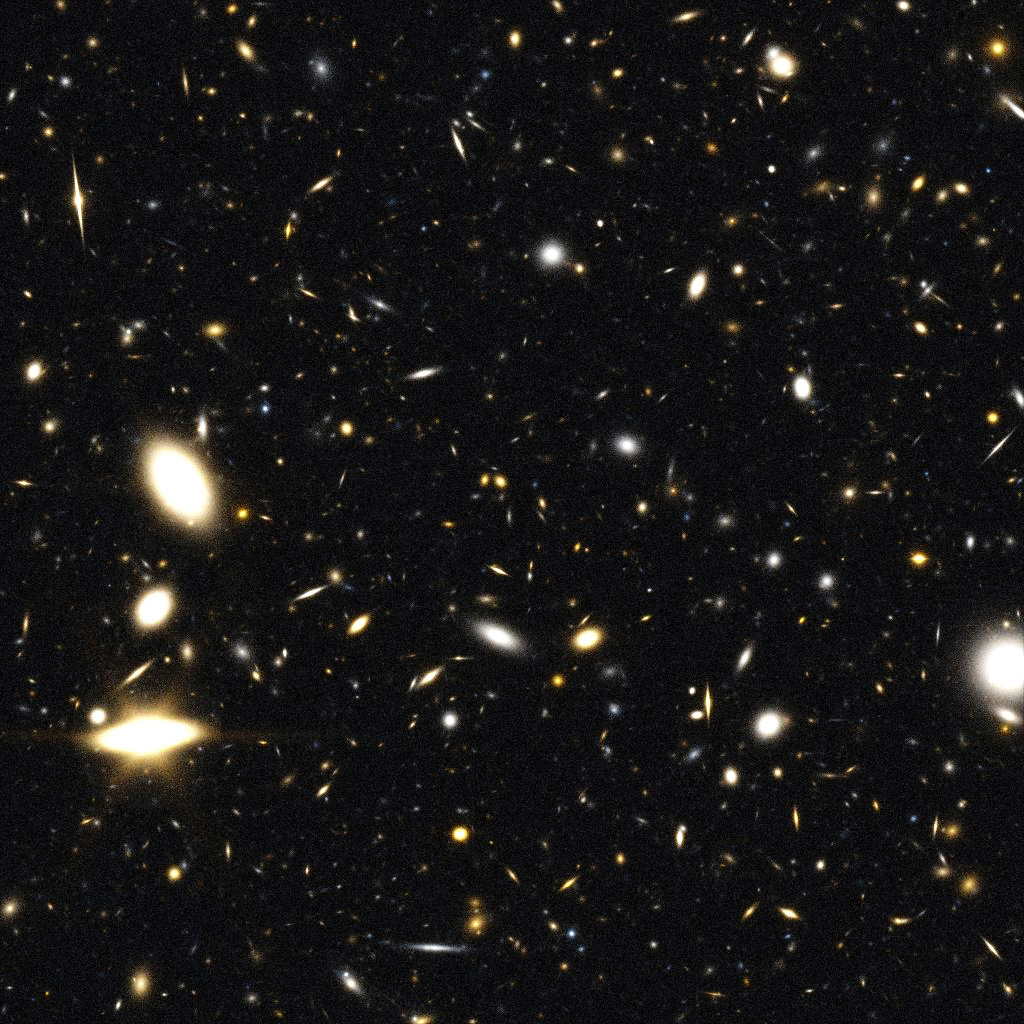
\includegraphics[width=0.75\textwidth]{plots/opo0220a.jpg}
    \caption{An image of galaxies from the James Webb Space Telescope, showing regions of high matter density and regions of low matter density.}
    \label{fig:galaxy_map}
\end{figure}
\begin{figure}[ht]
    \centering
    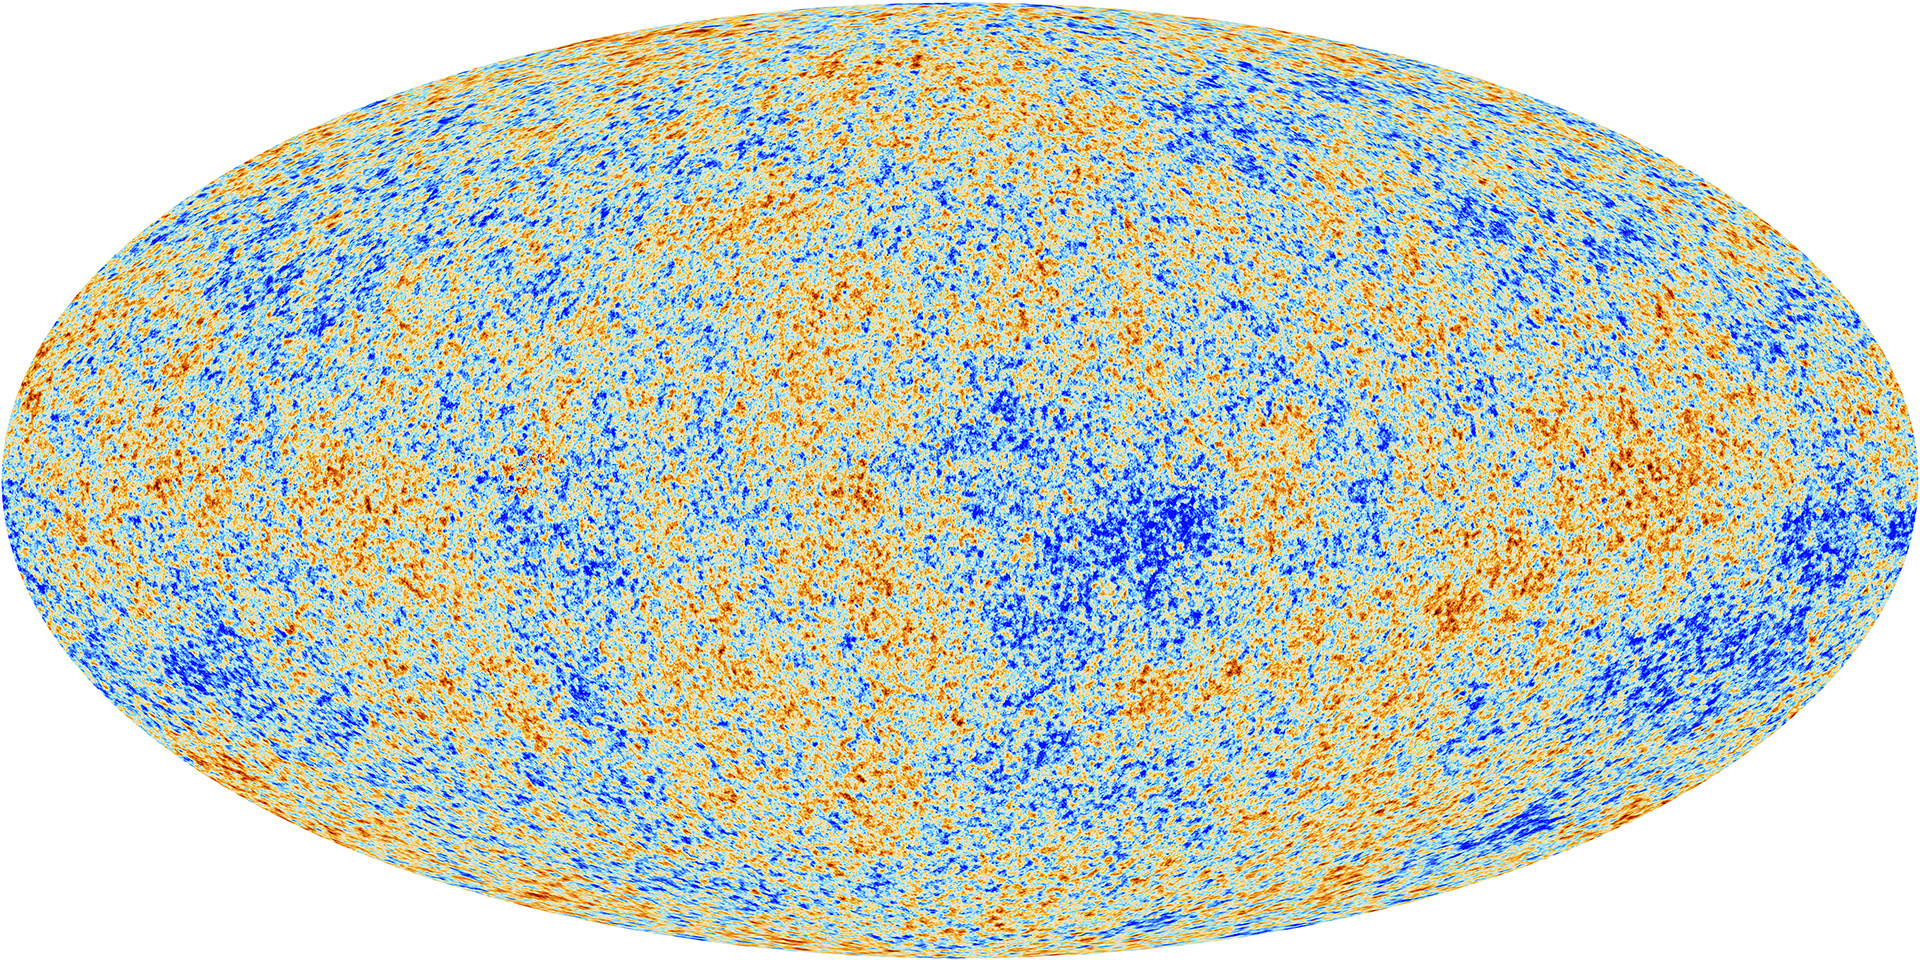
\includegraphics[width=0.75\textwidth]{plots/Planck_CMB.jpg}
    \caption{CMB TT power spectrum, emphasizing the scale of anisotropies.}
    \label{fig:cmb_tt_map}
\end{figure}

With Edwin Hubble's discovery of the expanding universe, any metric assigned to the universe must include homogeneous spatial expansion. Together with the above assumptions results in the FLRW metric.
\begin{equation}
    g = \text{diag}(-1,a^2,a^2,a^2)
\end{equation}
To perturb this metric around a homogenous universe, it requires two fields. The first, denoted $\Psi$, is the newtonian gravitational potential. Because newtonian gravity works in the non-relativistic limit, it enters the time component of the metric. The second field, denoted $\Phi$, represents spatial curvature perturbations. The perturbed metric is given by
\begin{equation}
    g = \text{diag}(-1-2\Psi,a^2(1-2\Phi),a^2(1-2\Phi),a^2(1-2\Phi))
\end{equation}
By computing the Christoffel symbols, one finds
\begin{equation}
    \begin{split}
        \Gamma^i_{00} = \frac{1}{a^2}\partial_i\Psi \\
        \Gamma^i_{0j} = \delta_{ij}(H+\dot\Phi) \\
        \Gamma^i_{jk} = (\delta_{ij} \partial_k + \delta_{ik}\partial_j - \delta_{jk}\partial_i)\Phi
    \end{split}
\end{equation}
Given Einstein's field equations and the perturbed FLRW metic, one can find the Friedman equations. The first comes from the 00 component of Einstein's field equations.
\begin{equation}
    H^2(t) = \frac{8\pi G}{3}\left(\rho + \frac{\Lambda}{8\pi G}\right) - \frac{k}{a^2}
\end{equation}
What can be done with this is to convert the curvature $k$ and the cosmological constant $\Lambda$ into densities as well, denoted $\rho_k$ and $\rho_\Lambda$ respectively. If those terms are absorbed into $\rho$, one finds
\begin{equation}
    H^2(t) = \frac{8\pi G}{3}\rho
\end{equation}
and the critical density is defined by the density associated with $H_0$,
\begin{equation}
    H_0^2 \equiv \frac{8\pi G}{3}\rho_{\text{crit}}
\end{equation}
Whats neat about this formulation with is that the value of the density today can tell us about the geometry of the universe. If $\rho>\rho_{\text{crit}}$ the curvature is positive (de Sitter geometry). If $\rho<\rho_{\text{crit}}$ the curvature is negative (anti-de Sitter geometry). If $\rho=\rho_{\text{crit}}$, the universe is flat. If we define the relative densities by
\begin{equation}
    \Omega_i = \frac{\rho_i}{\rho_\text{crit}}
\end{equation}
The relation becomes
\begin{equation}
    \Omega + \Omega_k = 1 
\end{equation}
Meaning if the non-curvature relative densities are less than 1, then the universe is curved with sign equal to the sign of $\Omega_k$.

The second Friedman equation comes from the trace of Einstein's equation.
\begin{equation}
    \frac{\ddot a}{a} = -\frac{4\pi G}{3}(\rho + 3P)
\end{equation}
In cosmology, there are other distances which can be more useful than the distance given by the FLRW metric. 
In the FLRW metric the distance between two points grows in time. 
We can avoid this by defining the \textit{comoving distance} in which distances remain fixed through time. 
If we look at a coordinate function $x^\mu$ at $t=t_0$, at a later time the coordinate function can be written as $x^\mu \rightarrow a(t) x^\mu$, thus by dividing by the scale factor $a(t)$ we can define the comoving coordinates as

\begin{equation}
    \chi = \int\limits^{t}_{t_0} \frac{1}{a(t')} dt'
\end{equation}

with the standard Minkowski metric. This can be taken a step further by determining how far light has travelled since $t=0$
\begin{equation}
    \eta = \int\limits^t_0 \frac{1}{a(t')}dt'
\end{equation}

Since we can't see anything beyond this distance, it is often called the \textit{comoving horizon}. 
There is one last useful distance to define, the \textit{angular distance} which is inferred by the angle subtended by two objects. 
This relates distances to the geometry discuss in the first section where the measured distance will be the radial distance $D$

\begin{equation}
    D_A = \left\{ \begin{array}{cc}
        R & K=0 \\
        R\sin(D/R) & K>0 \\
        R\sinh(D/R) & K<0
    \end{array}
    \right.
\end{equation}
\subsection{Cosmic Constituents of the Universe}
While we have made sense of the curvature density $\Omega_k$, there is still this mysterious $\Omega$ we see, which is a sum over other objects comprising the universe. Each of these objects are classified by their energy-momentum tensor and equation of state, defined by
\begin{equation}
    w_s = \frac{\mathcal{P}_s}{\rho_s}
\end{equation}
where $\mathcal{P}$ is the pressure and $\rho$ the density
\subsubsection{Radiation}
Radiation is defined to have 0 rest mass, and thus its energy-momentum is given by
\begin{equation}
    T = \text{diag}(\rho_\gamma, \rho_\gamma/3, \rho_\gamma/3, \rho_\gamma/3)
\end{equation}
(this can also be derived from Bose-Einstein statistics) Thus it has an equation of state $w_\gamma=1/3$. 

At one point, before recombination, radiation was the dominant component of the universe. As the universe cooled, the radiation was absorbed by the atoms forming until matter was the dominant. This formed the CMB which we measure today. Additionally, the CMB forms a nice black body, and thus the temperature can be found by measuring the emitted frequencies.
\subsubsection{Baryons}
Baryons are all non-relativistic particles which interact electromagnetically (so it excludes dark matter, but includes nuclei, electrons, etc.). Thus, its energy-momentum is given by
\begin{equation}
    T = \text{diag}(\rho_b,0,0,0)
\end{equation}
so its equation of state is given by $w=0$.
\subsubsection{Dark Matter}
Dark matter has the same energy-momentum as baryons, and thus the same equation of state. The main reason for the separation between Baryons and dark matter is that, experimentally, we can see baryons directly by imaging, but we cannot see dark matter. We can, however, see the gravitational effects of dark matter.
\subsubsection{Neutrinos}
Neutrinos are a special type of matter. They are relativistic $w=1/3$ but not radiation. Their energy-momentum can be computed the same way as for photons, but using Fermi-Dirac statistics. The density is thus
\begin{equation}
    \rho_\nu = \frac{21}{8}\left(\frac{T_\nu}{T}\right)^4\rho_\gamma
\end{equation}
\subsubsection{Dark Energy}
Dark energy is a special component of the universe. It is like a cosmological constant, and thus the energy momentum tensor is
\begin{equation}
    T = \text{diag}(\rho_\Lambda,-\rho_\Lambda,-\rho_\Lambda,-\rho_\Lambda)
\end{equation}
as such, its equation of state is $w=-1$

\section{General Relativity}

To align with my interest I will write this section from a mathematical perspective and give a physics interpretation after. In this section, I will derive Einstein's field equation. First starting with defining smooth structures on a manifold. Afterwards I move into curvature before using the Bianchi identity on the Riemann tensor to derive the equation governing General Relativity. I will also discuss some properties of Einstein's Field Equation.
\subsection{Smooth Manifolds}
The basic structure of our universe according to general relativity is that the universe is a smooth 4-manifold. This already contains a lot of information so lets break it down.
To begin, we start with defining a topological manifold. Given a space $X$ with topology $\tau$, $X$ is an $n$ dimensional topological manifold if
\begin{itemize}
	\item $X$ is Hausdorff. For each $p,q \in X$ there exists neighborhoods $p\in U$, $q\in V$, $U,V\in \tau$ such that $U \cap V = \empty$.
	\item $X$ is second countable. There exists a countable basis for the topology $\tau$.
	\item $X$ is locally Euclidean. For all $U\in\tau$ there exists a homemorphism $\phi:U\rightarrow V$ such that $V\subset \mathbb{R}^n$.
\end{itemize}
The last condition is one that hints at a differentiable structure becuase of known calculus in $\mathbb{R}^n$. To solidify this, consider the pair $(U,\phi)$ called a chart. Given two charts $(U,\phi)$ and $(V,\psi)$ with $U\cap V \neq \empty$, we can create the transition map $\psi \circ \phi^{-1}:\phi(U\cap V) \rightarrow \psi(U\cap V)$. The two charts are smoothly compatible if $U\cap V=\empty $ or the transition map is a homeomorphism.

\subsection{Curvature}
\subsection{Einstein's Field Equation}

Suppose we have a (semi-) Riemannian manifold $M$ with metric $g$ and tangent bundle $TM$. An \textit{affine connection} is a map
\[ \Gamma (TM) \times \Gamma (TM) \rightarrow \Gamma (TM) \]
\[ (X,Y) \rightarrow \nabla_X Y \]
That is, it parallel transports the vector field $Y$ along the connection $\nabla$ in the direction of vector field $X$. From this, we can write the affine geodesic equation for a path $\gamma(t)$
\[ \nabla_{\dot\gamma} \dot\gamma(t) = 0 \]
Thus, a geodesic is a path such that its tangent vector is parallel translated. Since we observe our world with coordinates, in physics it is often more instructive to work this out in a specific set of coordinates $x^\mu$. Thus this can be written as
\[ \ddot{\gamma}^\mu + \Gamma^{\mu}_{\rho\lambda}\dot{\gamma}^\rho \dot{\gamma}^\lambda  \]

In a curved spacetime, conservation of energy is written
\[ \nabla^\mu T_{\mu\nu} = 0\]
When deriving Einstein's equation, we want to find a divergence-less tensor that depends only on the geometry. The following procedure follows closely one would to find the classical Yang-Mills equation for gauge fields. The Riemann curvature is anti-symmetric in the first two lower indices, so the Riemann tensor is like a GL(TM) valued differential 2 form, and the bianchi identity is
\[ d_{\nabla} R = 0 \]
Explicitely writing this becomes
\[ \nabla_{\alpha} R^{\alpha}_{\beta\gamma\delta} + \nabla_{\beta}R^{\alpha}_{\gamma\alpha\delta} + \nabla_{\gamma}R^{\alpha}_{\alpha\beta\delta} = 0 \]
\[ \nabla_{\alpha} R^{\alpha}_{\beta\gamma\delta} + \nabla_{\beta}R^{\alpha}_{\gamma\alpha\delta} - \nabla_{\gamma}R^{\alpha}_{\beta\alpha\delta} \]
\[ \nabla_{\alpha}R^{\alpha}_{\beta\gamma\delta} + \nabla_{\beta}R_{\gamma\delta} - \nabla_{\gamma}R_{\alpha\delta} \]
Multiplying by $g^{\beta\delta}$ and doing some relabelling/contractions of internal indices we find
\[ \nabla^\alpha(R_{\gamma\alpha}-\frac{1}{2}g_{\gamma\alpha}R) \equiv \nabla^{\alpha}G_{\gamma\alpha} = 0 \]
There is one more divergencless tensor, the metric tensor $g_{\mu\nu}$, so we can write
\[ G_{\mu\nu} - \Lambda g_{\mu\nu} = 8\pi\kappa T_{\mu\nu} \]

\subsection{Gauge Choice}
\subsection{Scalar-Vector-Tensor Decomposition}

Our universe, as described above, is a real valued 4 dimensional space, $\mathbb{R}^4$. Suppose that we can separate the universe into a spacial part and a temporal part $\mathbb{R}^4 \mapsto \mathbb{R} \times S$ where $S$ is some $3$-manifold. Under such a decomposition, the metric decomposes as (with comoving time as the time coordinate)
\[ g = a^2(\tau)\left( g_{00}d\tau d\tau + g_{0i}d\tau dx^{i} + g_{ij} dx^{i}dx^{j} \right) \]
The three parts are as follows:
\begin{itemize}
    \item $g_{00}$ has degrees of freedom (DOF) of a scalar. This is the scalar portion of the decomposition.
    \item $g_{0i}$ has DOF of a vector. This is the (co)vector portion of the decomposition.
    \item $g_{ij}$ has DOF of a rank 2 tensor. This is the tensor portion of the decomposition.
\end{itemize}
The metric, however, is a special case of a symmetric rank 2 tensor. For antisymmetric tensors the only change is that rather than the product $dx^\mu dx^\nu$, we need the exterior product $dx^\mu \wedge dx^\nu$. This means the temporal component/scalar component is 0 for antisymmetric tensors. Since any rank 2 tensor can be decomposed to a symmetric and an antisymmetric part, these two decompositions are sufficient for decomposing any rank 2 tensor. 

We can take this even further. Note that a vector can be decomposed into a divergence part and a dual part
\[ v^i = g^{ij}\partial_j f + g^{ij} \underbrace{w_{jk}\star (dx^{i} \wedge dx^{j})}_{\equiv \hat{w}_j} \]
\[ \Rightarrow v^i = (\partial^j f + \hat{w}^j) \]
Also, any rank 2 tensor can be written as the sum of a trace and a traceless part.
\section{$\Lambda$CDM: The Standard Model of Cosmology}


\subsection{The FLRW Metric and Dark Energy}
In general, metrics allow one to attribute distances between points in a space as $d = g_{\mu\nu}x^\mu x^\nu$. 
The `flat' metric for relativity is the \textit{Minkowski metric} given by $\text{diag}(-1,1,1,1)$, however, a metric to describe the expanding universe is given by the \textit{FLRW metric} by $d^2 = t^2-a^2(t)s^2$ with $s^2$ the standard Euclidean distance in $\mathbb{R}^3$. 
What is immediately appearent from the FLRW metric is that spacial slices of the $d=4$ spacetime remain curvature free under the expansion of the universe describe by the scale factor $a^2(t)$.

In cosmology, there are other distances which can be more useful than the distance given by the FLRW metric. 
In the FLRW metric the distance between two points grows in time. 
We can avoid this by defining the \textit{comoving distance} in which distances remain fixed through time. 
If we look at a coordinate function $x^\mu$ at $t=t_0$, at a later time the coordinate function can be written as $x^\mu \rightarrow a(t) x^\mu$, thus by dividing by the scale factor $a(t)$ we can define the comoving coordinates as

\begin{equation}
    \chi = \int\limits^{t}_{t_0} \frac{1}{a(t')} dt'
\end{equation}

with the standard Minkowski metric. This can be taken a step further by determining how far light has travelled since $t=0$
\begin{equation}
    \eta = \int\limits^t_0 \frac{1}{a(t')}dt'
\end{equation}

Since we can't see anything beyond this distance, it is often called the \textit{comoving horizon}. 
There is one last useful distance to define, the \textit{angular distance} which is inferred by the angle subtended by two objects. 
This relates distances to the geometry discuss in the first section where the measured distance will be the radial distance $D$

\begin{equation}
    D_A = \left\{ \begin{array}{cc}
	    R & K=0 \\
	    R\sin(D/R) & K>0 \\
	    R\sinh(D/R) & K<0
    \end{array}
    \right.
\end{equation}

When describing the structure of the universe, I will make a few assumptions (which hold up to small perturbations):

\begin{itemize}
    \item Homogeneity. The cosmology describing the universe does not depend on location.
    \item Isotropy. The cosmology describing the universe does not depend on location.
\end{itemize}

These two conditions for what is sometimes referred to as \textit{the cosmological principle}. 
In general, they don't hold on small scales, however averaging over a sufficiently large distance these assumptions give an accurate description. 
The isotropy condition means that the universe should have 0 net momentum, and by assumming the universe is smooth the energy-momentum tensor can be written

\begin{equation} T^\mu_\nu = \left(
\begin{array}{cccc}
    -\mathcal{E} & 0 & 0 & 0 \\
    0 & \mathcal{P} & 0 & 0 \\
    0 & 0 & \mathcal{P} & 0 \\
    0 & 0 & 0 & \mathcal{P}
\end{array}
\right)
\end{equation}

The usual conservation law holds

\begin{equation}
    \nabla_\mu T^{\mu}_{\nu} = 0 \Rightarrow \partial_t \mathcal{E} + \frac{\dot a}{a}(3\mathcal{E} + 3\mathcal{P}) = 0
\end{equation}

We can use the geodesic equation to examine how the energy of the massless particles evolves through time. 

If we examine the $00$ component of Einstein's Field Equation, the result is the \textit{first Friedman equation} (note that $\rho$ is shorthand for $\sum_i\rho_i$ and $R(G)$ to note that $R$ depends on the geometry of spaceial slices)

\begin{equation}
    H^2(a) + \frac{1}{a^2 R^2(G)} = \frac{8\pi G}{3}\rho
\end{equation}

We can interpret the second term on the left (which is spacial curvature) as some density asociated with the curvature $\rho_k$. If we divide by $\rho_{\text{crit}}$ at $z=0$ / $a=1$ we find the usual form. 

\begin{equation}
    \omega + \omega_k = 1 
\end{equation}

The second Friedman equation comes from the trace of Einstein's equation.

\begin{equation}
    \frac{\ddot a}{a} = -\frac{4\pi G}{3}(\rho + 3P)
\end{equation}

\subsection{informal notes}
perfect fluid approximation: treating galaxies as particles of a gas, the particles cluster at small scales and can the particle nature can be ignored.
The fluid of galaxies has stress-energy 

\begin{equation*}
    T = (\rho+p) u\otimes u + gp
\end{equation*}

with $u$ the 4-velocity and $g$ the metric tensor and $p$ the pressure and $\rho$ the mass-energy.

\chapter{Measurement of Weak Lensing and the Cosmic Microwave Background}
\section{Weak Lensing}
In general, contemporary weak lensing surveys measure the light emitted from galaxies in two components: galaxy position and galaxy shear. In the following sections, the theoretical base for cosmological weak lensing surveys are described. However, before discussing the two relevant observables, one needs to formalize the concept of weak lensing.
\begin{figure}[ht]
	\centering
	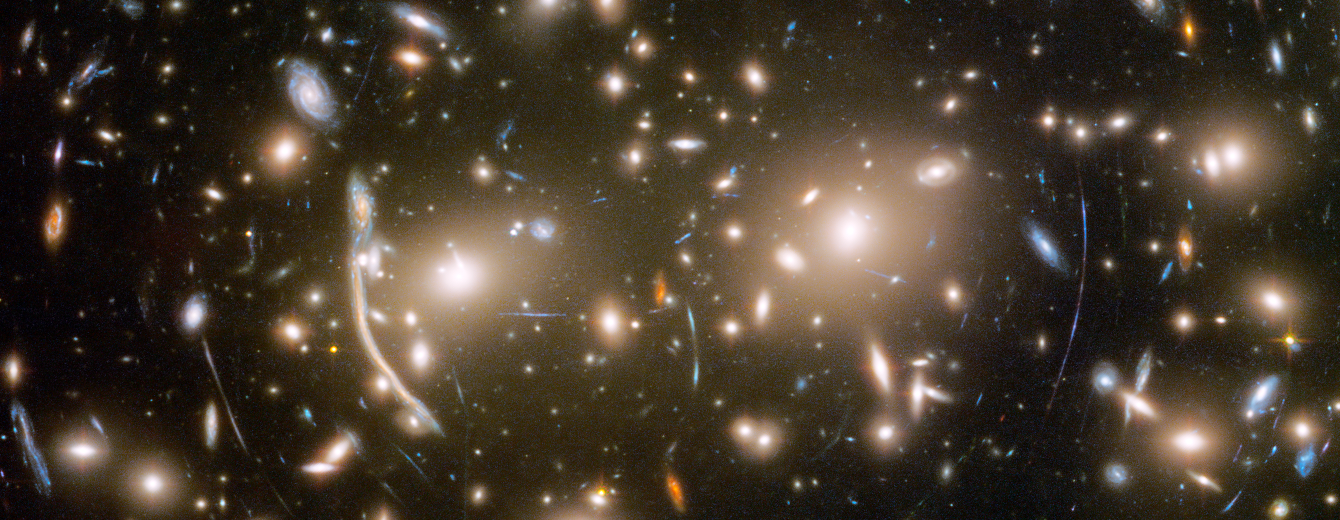
\includegraphics[width=\textwidth]{plots/hubble_weak_lensing.png}
	\caption{Image of weak lensing taken by the Hubble Space Telescope~\cite{hubble_lensing}.}
	\label{fig:weak_lensing}
\end{figure}
\subsection{The Linear Matter Power Spectrum}
As we have seen before, we consider deviations from the FLRW metric using the scalar fields $\Phi$ and $\Psi$. In the absence of anisotropic stress, $\Phi=-\Psi$, which we will assume here for demonstration (one can use codes such as CAMB or CLASS to do computations including anisotropy if desired). 

Throughout time in the universe, we consider there to be three distinct epochs or regions~\cite{scott_dodelson_modern_2021}:
\begin{itemize}
	\item The super-horizon region, or the region before inflation where radiation dominates
	\item The horizon-crossing region, or the region during inflation where the universe transfers from radiation to matter domination
	\item The sub-horizon region, or the region of after rapid inflation where matter dominates
\end{itemize}
Additionally, the formation of matter inhomogeneity comes from gravitational instability, the idea that primordial curvature perturbations in the super-horizon grew to form small matter density contrasts which grew after crossing the horizon. After the rate of inflation slowed, gravitational forces caused clusters of matter to become the galaxies and clusters we see today.

This gives us a blueprint for writing the matter power spectrum. We have the primordial curvature perturbation $\mathcal{R}$ which source the initial matter inhomogeneity that formed late-time large scale structure. Thus, we can write it as
\begin{equation}
	\mathcal{R} = \frac{5}{3}\Phi_{\text{large-scale}}(k,a_{\text{late}})\,.
\end{equation} 
Additionally, we have a transfer function which describes the transition from radiation to matter domination, defined as
\begin{equation}
	T(k) = \frac{\Phi(k,a_{\text{late}})}{\Phi_{\text{large-scale}(k,a_{\text{late}})}}\,.
\end{equation}
And we have a growth factor, defined as the linear growth of matter density contrast during matter domination, defined as
\begin{equation}
	D_+(a) = a \frac{\Phi(k,a)}{\Phi(k,a_{\text{late}})}\,.
\end{equation}
Thus we can write the gravitational potential at all times as
\begin{equation}
	\Phi(k,a) = \frac{3}{5a}\mathcal{R}(k)T(k,a)D_+(a)\,.
\end{equation}
This together with the Poisson equation for the matter density contrast field gives the equation
\begin{equation}
	\delta_m(k) = \frac{2k^2a}{3\Omega_mH_0^2}\Phi(k,a)\,,
\end{equation}
\begin{equation}
	\delta_m(k) = \frac{2}{5}\frac{k^2}{\Omega_mH_0^2}\mathcal{R}(k)T(k,a)D_+(a)\,,
\end{equation}
The power spectrum of an observable is defined as the two-point correlation function of the observable in Fourier space.
\begin{equation}
	P_\mathcal{O}(k) = \langle \mathcal{O}(k)\mathcal{O}(k) \rangle\,.
\end{equation}
Thus, the linear matter power spectrum (because we restricted the matter density contrast field to linear order terms in the perturbation) is given by
\begin{equation}
	\begin{split}
		P_m^{L}(k,a) = \frac{8\pi^2}{25 \Omega_m^2 H_0^4} A_s D_+^2(a)T^2(k)\frac{k^{n_s}}{k_p^{(n_s-1)}}\,.
	\end{split}
\end{equation}

\subsection{Galaxy Density}
In practice, we cannot measure the matter power spectrum; Dark matter prohibits direct measurement. Instead, one must determine observables which trace the matter distribution in the universe. The most natural option is to observe the galaxy distribution. However, large scale structures and galaxies provide many sources for non-linearities in the power spectrum and result in a non-trivial relation between the two. By taking certain data selection criteria, one can cut out the non-linear contributions. The relation between the galaxy and matter power spectra are then related by the linear bias factor.
\begin{equation}
	\begin{split}
		\delta_g(k) &= b_1 \delta_m(k) \\
		P_g(k,a) &= (b_1)^2P_m^L(k,a)\,.
	\end{split}
\end{equation}
Realistically, in galaxy surveys, we do not have access to exact redshifts for each observed galaxy. Rather, an image is taken of the sky in multiple color bands, from which the redshift is determined. This procedure is called photometric redshift. To account for this, one can attempt to redefine the galaxy power spectrum. First, we define the distribution of distances, as
\begin{equation}
	W(\chi) = \frac{1}{N_g}\frac{dN_g}{d\chi}\,.
\end{equation}
The procedure for determining this distribution will be discussed in sections~\ref{sec:dz} and~\ref{sec:IA}. This allows us to simply write the projected density contrast as
\begin{equation}
	\Delta_g = \int\limits_0^\infty W(\chi)\delta_g(x,\tau)d\chi\,.
\end{equation}
To complete this discussion, we will make some approximations. The first is that we will only consider small scales for which $\sin(\theta)\sim \theta \sim 1/l$ where $l$ is the Fourier conjugate of $\theta$. The second is the limber approximation, which states that, as long as the galaxy power spectrum $P_g$ slowly varies over the region $\Delta k \sim 1/l\chi$, we approximate is as a constant. These approximations greatly simplify the integrals required when computing the power spectrum of the Fourier transformed $\Delta_g$. This power spectrum is called the angular power spectrum. Considering the approximations above and computing the Fourier transform, one finds an angular power spectrum of
\begin{equation}
 	C_g(l) =\int \frac{1}{\chi^2}W^2(\chi)P_g(k=(l+1/2)/\chi,\eta) d\chi\,.
\end{equation} 
\subsection{Galaxy Shear}
Photons move on null geodesics, thus $d\chi = -d\eta$, where $\eta$ is the conformal time and $\chi$ is the conformal distance. This tells us that, through some changes of variables, $dx^i/d\chi = -\hat{p}^i$ (for photons and other massless particles). Thus, under lensing, the difference between the observed and true positions within the source plane is given by
\begin{equation}
	\chi\mathbf{\theta}^i = x_\perp^i = -\int\limits_0^\chi \hat{p}^i_\perp(\chi'') d\chi''\,.
\end{equation}
The goal is to write this as a function of the potential only. Thus, we look to compute $d\hat{p}^i/dt$.
\begin{equation}\label{eq:dp-hat-dt}
	\begin{split}
		\frac{d\hat{p}^i}{dt} %=& \frac{d}{dt}\frac{1}{p}p^i \\
		=& \frac{1}{p^2}(\dot{p}^i p - \dot{p}p^i)\,.
	\end{split}
\end{equation}
By computing $\dot p^i$, one can find $\dot p$ as well:
\begin{equation}
	\begin{split}
		\frac{dp^i}{d\lambda} %=& \frac{d}{d\lambda}\left(aP^i(1+\Phi)\right) \\
		=& P^i\frac{d}{d\lambda}(a(1+\Phi)+(1+\Phi)a\frac{d}{d\lambda}P^i\,.
	\end{split}
\end{equation}
Also, $d/d\lambda = P^\mu \partial_\mu$, so the first term becomes
\begin{equation}
	\begin{split}
		P^i\frac{d}{d\lambda}(a(1+\Phi)) %&= P^iP^\mu \partial_\mu(a(1+\Phi)) \\
		%&= P^iP^0(\dot a + a\dot\Phi + \dot a \Phi) + a P^iP^j \partial_j\Phi \\
		&= a P^i (P^0(H+\dot\Phi +H\Phi) + P^j\partial_j\Phi)\,. \\
	\end{split}
\end{equation}
The second term is evaluated by using the geodesic equation up to first order in the perturbations $\Phi$ and $\Psi$.
\begin{equation}
	\begin{split}
		\frac{d}{d\lambda}P^i &= -\Gamma^i_{\mu\nu}P^\mu P^\nu \\
		%&= -(P^0)^2\frac{1}{a^2}\partial^i\Psi - 2\delta^{i}_{j}(H+\dot\Phi)P^0P^j + 2P^iP^j\partial_j\Phi - P^jP_j\partial^i\Phi \\
		%&= -E(1-\Psi)\left( \frac{E}{a^2} \partial^i\Psi + \frac{1}{a}2p^i(1-\Phi)(H+\dot\Phi) - \frac{2}{a^2E}p^ip^j\partial_j\Phi + \frac{p^2}{a^2E} \partial^i\Phi \right) \\
		&= -E\left( \frac{E}{a^2} \partial^i\Psi + \frac{1}{a}2p^i(1-\Phi-\Psi)(H+\dot\Phi) - \frac{2}{a^2E}p^ip^j\partial_j\Phi + \frac{p^2}{a^2E} \partial^i\Phi \right)\,.
	\end{split}
\end{equation}
Plugging everything back in, and only keeping terms to linear order, one gets
\begin{equation}
	\begin{split}
		%=& aP^i(H+\dot\Phi+H\Phi) + aP^iP^j\partial_j\Phi \\
		%& - \frac{E}{a}\partial^i\Psi - 2p^i(H+\dot\Phi) + \frac{2}{aE}p^ip^j \partial_j\Phi - \frac{p^2}{aE}\partial^i\Phi \\
		\frac{dp^i}{dt} %=& p^i(1-\Phi)(H+\dot\Phi+H\Phi) + (1-\Phi)^2p^ip^j\partial_j\Phi \\
		%& - \frac{E}{a^2}\partial^i\Psi -\frac{2p^i}{a}(H+\dot\Phi) + \frac{2}{a^2E}p^ip^j \partial_j\Phi - \frac{p^2}{a^2E}\partial^i\Phi \\
		%=& p^i(H+\dot\Phi) + \frac{p^ip^j}{aE}\partial_j\Phi \\
		%& - \frac{E}{a}\partial^i\Psi -2p^i(H+\dot\Phi) + \frac{2}{aE}p^ip^j \partial_j\Phi - \frac{p^2}{aE}\partial^i\Phi \\
		=& -p^i(H+\dot\Phi)- \frac{1}{aE}\left(p^ip^j\partial_j\Phi - p^2\partial^i\Phi\right) -\frac{E}{a}\partial^i\Psi\,.
	\end{split}
\end{equation}
The time derivative of the modulus of the momentum, $p$, is then given by
\begin{equation}
	\begin{split}
		\frac{dp}{dt} =& \frac{d}{dt}\sqrt{\delta_{ij}p^ip^j} = \frac{1}{p}\delta_{ij}\dot p^i p^j \\
		%=& -p(H+\dot\Phi) - \frac{p}{aE}(p^i\partial_i\Phi - pp^i\partial^i\Phi) - p^i\frac{E}{ap}\partial^i\Psi \\
		=& -p(H+\dot\Phi) - \hat{p}_i\frac{E}{a}\partial^i\Psi\,.
	\end{split}
\end{equation}
Now, putting everything together, plugging these results into eq~\ref{eq:dp-hat-dt} gives
\begin{equation}
	\begin{split}
		\frac{d\hat{p}^i}{dt} %=& -\hat{p}^i(H+\dot\Phi)- \frac{1}{aEp}\left(p^ip^j\partial_j\Phi - p\partial^i\Phi\right) -\frac{E}{ap}\partial^i\Psi + \hat{p}^i\left( (H+\dot\Phi) + \hat{p}_i\frac{E}{ap^2}\partial^i\Psi \right) \\
		=&  \frac{E}{ap}\left( \frac{p^2}{E^2}\partial_j\Phi - \partial_j\Psi \right)(\delta^{ij}-\hat{p}^i\hat{p}^j)\,.
	\end{split}
\end{equation} 
Going back to the photon scenario, where $E=p$, this simplifies to
\begin{equation}
	\frac{d\hat{p}^i}{dt} = \frac{1}{a}\left( \partial_j\Phi - \partial_j\Psi \right)(\delta^{ij}-\hat{p}^i\hat{p}^j)\,.
\end{equation}
Interestingly, $\delta^{ij}-\hat p^i \hat p^j$, is the projection operator of the $j$-th direction onto the $i$-th. So, if we orient our axes so that the photon approximately travels along the $j$-th direction, we can sum of $i$ and $k$ so that the orthogonal components of the momentum are evaluated by
\begin{equation}
	\frac{d\hat{p}^i_\perp}{d\chi} = - a \frac{d\hat{p}^i_\perp}{dt} = -\partial_i(\Phi-\Psi)
\end{equation}
In the absence of anisotropic stress (like in the late universe where weak lensing is measured), $\Phi=-\Psi$ and 
\begin{equation}
	\frac{d\hat{p}^i_\perp}{d\chi} -2\partial_i\Phi\,.
\end{equation}
Integrating this equation gives
\begin{equation}
	\hat p_\perp (\chi'') = -2\int\limits_0^{\chi''}\partial_i\Phi(\chi') d\chi' + C_i\,,
\end{equation}
where the constant $C_i$ comes from integrating a derivative, where it is only defined up to a constant. Now, plugging this back in one finds
\begin{equation}
	\mathbf{\theta}^i = \frac{2}{\chi}\int\limits_0^\chi \int\limits_0^{\chi''}\partial_i\Phi(\chi') d\chi' d\chi'' - C_i\,.
\end{equation}
In the absence of lensing, this should reduce to $\mathbf{\theta}^i = \theta_0$, the true source position. Hence $C^i=\theta^i_0$ and the total deflection angle is given by
\begin{equation}
	\begin{split}
		\Delta\theta^i =& \frac{2}{\chi}\int\limits_0^\chi \int\limits_0^{\chi''}\partial_i\Phi(\chi') d\chi' d\chi''\\
		=& \frac{2}{\chi}\int\limits_0^\chi \partial_i\Phi(\chi') (\chi-\chi') d\chi'\,.
	\end{split}
\end{equation}
Finally, since $x^i=\chi\theta^i$, $\partial_i = \partial_{\theta^i}/\chi$. Introduce the \textit{lensing potential} defined by
\begin{equation}
	\begin{split}
		\Delta\theta^i =& \frac{\partial}{\partial \theta^i}\psi_L(\theta) \\
		\psi_L(\theta) =& 2\int\limits_0^\chi \frac{1}{\chi'}\Phi(\chi') \left(1-\frac{\chi'}{\chi}\right) d\chi'\,.
	\end{split}
\end{equation}
This result is great, but it's not very experimentally illuminating. Similar to the galaxy versus matter power spectrum, the absence of the observation of dark matter means we cannot reliably determine the potential $\Phi$. Again, an attempt to relate the lensing potential to some property of galaxies can give us a measurable quantity. Lensing distorts the shape of the galaxies (see figure~\ref{fig:weak_lensing}), where we assume all galaxies are elliptical. Define the galaxy shape tensor by
\begin{equation}
	q_{ij} \equiv \frac{1}{F}\int I\theta^i\theta^j d\theta^i d\theta^j\,.
\end{equation}
This integral is symmetric under $i \leftrightarrow j$. Writing this as a matrix gives
\begin{equation}
	q_{ij} = \frac{1}{2} \text{tr}(q) \left( 
	\begin{array}{cc}
	1+\epsilon_1 & \epsilon_2 \\
	\epsilon_2 & 1-\epsilon_1
	\end{array}
	\right)\,.
\end{equation}
Shape distortion occurs when the deflection angle is not constant across a galaxy. We can look at the transformation tensor as
\begin{equation}
	A_{ij} \equiv \frac{\partial \theta^i_S}{\partial\theta^j} = \left( 
	\begin{array}{cc}
	1+\kappa - \gamma_+ & -\gamma_\times \\
	-\gamma_\times & 1+\kappa+\gamma_+
	\end{array}
	\right) = \delta_{ij}+\psi_{ij}\,.
\end{equation}
Within this tensor, the $\gamma_+$ and $\gamma_-$ terms represent shear and $\kappa$ represents magnification and changes in galaxy light flux ($F$). The $E$-mode is given by
\begin{equation}
	E(l) = \left( \frac{l^il^j}{l^2} - \frac{1}{2}\delta^{ij} \right)(-\psi^{ij}(l))\,.
\end{equation}
Which relates to the shear components by
\begin{equation}
	\left(
	\begin{array}{c}
	\gamma_+ \\
	\gamma_\times
	\end{array}
	\right)
	=
	\left(
	\begin{array}{c}
	\cos(2\alpha_l) \\
	\sin(2\alpha_l)
	\end{array}
	\right)
	E(l)\,.
\end{equation}
This connects the observable shear to the theoretical lensing potential.
\subsection{Weak Lensing Correlation Functions}
In the previous two sections, we have derived two observables directly connected to cosmological theories. By observing the galaxies we can determine $\Omega_b$, $A_s$, $n_s$ and $H_0$. By observing shear, we can determine $\Omega_m$. The details of how to determine these parameters will be discussed in chapter 3. Together, these two can fully determine the values of the 5 $\Lambda$CDM parameters. These two quantities themselves are not observables. Using these two quantities, however, one can construct three different two-point correlation functions which are observable.

The first correlation function is the autocorrelation of galaxy density, called galaxy clustering. Given a density in a particular angular position, the correlation function can be interpreted as the likelihood of observing a similar density at another close position. The galaxy clustering correlation function is given by
\begin{equation}
	w_g(\theta) = \mathcal{F}(C_g(l)) = \frac{1}{2\pi}\int\limits_0^\infty l C_g(l) J_0(l\theta)dl\,,
\end{equation}
where $J_0$ is the 0-th Bessel function and $\mathcal{F}$ denotes the Fourier transform.

Next is the shear autocorrelation. In this case, there are two components of shear: the tangential shear $\gamma_+$ and the cross shear $\gamma_\times$. The cross correlation $\langle \gamma_+ \gamma_\times \rangle$ vanishes, and the remaining combinations are
\begin{equation}
	\begin{split}
		\langle \gamma_+\gamma_+ \rangle \pm \langle \gamma_\times \gamma_\times \rangle = \xi_\pm
	\end{split}
\end{equation}
\begin{equation}
	\xi_{+,-} = \frac{1}{2\pi}\int\limits_0^\infty l C_{EE}(l) J_{0,4}(l\theta)C_{EE}(l)dl\,.
\end{equation}

The final observable is the cross correlation between galaxy density and tangential shear. First, the angular power spectrum $C_{gE}(l)$ is given by
\begin{equation}
	C_{gE}(l) = \frac{3}{2}\Omega_mH_0^2 \int\limits_0^\infty \frac{1}{\chi a(\chi)}W_g(\chi)P_g(k,\eta) d\chi\,.
\end{equation}
\begin{equation}
	\gamma = \langle \Delta_g\gamma_+\rangle = -\frac{1}{2\pi}\int\limits_0^\infty l J_2(l\theta)C_{gE}(l)dl\,.
\end{equation}
The correlation function $\langle \Delta_g\gamma_\times\rangle$ vanishes in an isotropic universe.

\subsection{Systematics}
Up to now, we have neglected any systematics of the weak lensing observables. There are two distinct types of systematics that will be discussed in this section: The ones which affect the calculation of the correlation functions, and the ones which affect the correlation functions after they have been computed. The latter type of parameters are usually referred to as `fast' parameters, and it will become clear why that is in the next chapter. In the meantime, here is an explanation of the relevant systematics.
\subsubsection{Photometric Redshift Uncertainty}\label{sec:dz}
To compute the two-point correlation functions, one must determine the redshift distribution $W(\chi)$. This is a highly non-trivial task. To model the uncertainty in this distribution, one applies a constant shift to the redshift of observed galaxies.
\begin{equation}
	n_g(z) \mapsto n_g(z+\Delta z)
\end{equation}
The shift $\Delta z$ must be determined before one can compute the galaxy clustering and galaxy lensing correlation functions.
\subsubsection{Intrinsic Alignment of Galaxies}\label{sec:IA}
As can be seen in figure (fig), galaxy shapes are not completely random. In the absence of lensing, there is still some non-zero correlation between the shapes. This is referred to as Intrinsic Alignment~\cite{troxel_intrinsic_2015,scott_dodelson_modern_2021}. There are two models of intrinsic alignment that will be considered in this thesis: the Tidal Alignment Tidal Torquing (TATT) model~\cite{krause_dark_2021,blazek_beyond_2019} and the Non-linear Alignment (NLA) model. The TATT depends on the tidal tensor $s_{ij}$, which contains the information about tidal forces due to non-uniform gravitational fields. Tidal forces are a source of intrinsic alignment and shear (figure). The model is given by
\begin{equation}
	\gamma_{ij}^I = \underbrace{C_1s_{ij}}_{\text{tidal alignment}}+
	\underbrace{b_{TA}C_1(\delta_m\times s_{ij})}_{\text{density weighting}}+
	\underbrace{C_2\left( s_i^ks_{kj}-\frac{1}{3}\delta_{ij}s^2 \right)}_{\text{tidal torquing}}\,,
\end{equation}
where the coefficients $C_a$ are given by
\begin{equation}
	\begin{split}
		C_1 =& -\frac{A_1\bar{C}\Omega_m}{aG(z)}\left(\frac{1+z}{1+z_0}\right)^{\eta_1} \\
		C_2 =& 5\frac{A_2\bar{C}\Omega_m}{(aG(z))^2}\left(\frac{1+z}{1+z_0}\right)^{\eta_2}\,.
	\end{split}
\end{equation}
The TATT model reduces to the NLA model when $A_2=0=b_{TA}$.
\subsubsection{Galaxy Bias}
As discussed in the galaxy clustering section, we relate the galaxy and matter density by a bias parameter $b$. However, we can pick a fiducial value to relate the two
\begin{equation}
	\delta_{g,\text{fid}} = b_{\text{fid}}\delta_m
\end{equation}
then consider a multiplicative deviation:
\begin{equation}
	\delta_g = (b\cdot b_{\text{fid}})\delta_m = b\delta_{g,\text{fid}}\,.
\end{equation}
Thus, the parameter $b$ can be found to account for different galaxy biases. 

Galaxy bias is the first of many `fast' parameters. Since the bias is constant, it can be pulled out of the integral for the correlation functions, meaning it can be applied after the correlation function has been computed. The affected correlation functions are the galaxy clustering and galaxy-galaxy lensing.
\begin{equation}
	\begin{split}
		w^i(\theta) =& b_{(i)}^2w^i(\theta) \\
		\gamma^i_t(\theta) =& b_{(i)}\gamma_t^i(\theta)\,.
	\end{split}
\end{equation}
where $i$ denotes the redshift bin.
\subsubsection{Shear Calibration}
Observed shear is not a completely astrophysical phenomenon. For example, a major source of additional shear comes from the observation lens itself, where the observed galaxy shape is given by the true galaxy shape convolved with the point spread function of the lens~\cite{hirata_shear_2003,gillis_effects_2019}. This is usually modelled as a multiplicative correction to the shear components.
\begin{equation}
	\begin{split}
		\xi^{ij}_{\pm} =& (1+m^i)(1+m^j) \xi^{ij}_{\pm} \\
		\gamma^{ij}_t =& (1+m^j) \gamma_t^{ij}\,,
	\end{split}
\end{equation}
where $i$ and $j$ denote the source and lens bin respectively. The multiplicative shear calibration is also a fast parameter.
\subsubsection{Point Mass}
Currently, we are unable to model the contribution of small scales to the tangential shear~\cite{maccrann_controlling_2020}. The tangential shear can be written in terms of the surface mass density $\Sigma$ in the tangential direction:
\begin{equation}
	\gamma_t(R/D_A) = \frac{\bar\Sigma(0,R) - \Sigma(R)}{\Sigma_\mathrm{crit}} = \frac{\Delta\Sigma(R)}{\Sigma_\mathrm{crit}}\,.
\end{equation}
We can only model the tangential shear to $r_\mathrm{min}$, which allows us to write the point mass contribution (named for the $R^{-2}$ dependence) as
\begin{equation}
	\Delta\Sigma(R) = \Delta\Sigma^{\mathrm{model}}(R) + \frac{B}{R^2}\,.
\end{equation}
\subsubsection{Lensing Magnification}
In weak lensing, the intrinsic shape of galaxies also gets magnified. This effect is introduced as a parameter $C_l^i$ and is fixed experimentally.

%Additionally, DES added a non-physical parameter called $X_{\text{lens}}$ to resolve an inconsistency between two lensing samples, RedMaGiC and MagLim. In this thesis, we only consider $X_{\text{\lens}}=1$

\section{CMB}
Although CMB data is not used very much in this thesis, it is worth discussing the measurements qualitatively. The consensus among physicists and astronomers that the universe beyond the horizon was a hot, dense plasma. As such, the mean free path of photons was much shorter than it is today, and thus Compton scattering dominated photon dynamics in the early universe. As the universe cooled, atoms began to form in a process called recombination~\cite{scott_dodelson_modern_2021,hu_animations_nodate}. During this time, the universe was still opaque as photons scattered on the newly formed atoms. As the universe began to expand, the mean free path of photons increased and inter-atomic interactions decreased, meaning the atoms could be ionized by absorbing free photons in a process called reionization. The absorption of the photons caused the universe to become transparent. One can compute the optical depth of this transition from opaque to transparent as
\begin{equation}
	T = T_0(1-e^{-\tau_{\mathrm{rei}}})\,.
\end{equation}
$\tau_{\mathrm{rei}}$ concludes the introduction of cosmological parameters. $\tau_{\mathrm{rei}}$ can only be determined from CMB and is usually fixed in weak lensing analysis.

The CMB is a black body, meaning the intensity of the light can be used to determine the temperature according to the black body equation where $I \propto T^4$. The temperature, along with the $E$-mode polarization, gives three possible two point correlation functions: $TT$, $TE$, and $EE$.
\subsection{TT Power Spectrum}
\begin{figure}
    \centering
    \includegraphics[width=12cm]{plots/Planck_TT.png}
    \caption{Planck TT power spectrum}
    \label{fig:planck_tt}
\end{figure}
The TT power spectrum measures the anisotropies of the temperature field. Thus, it is better to consider it as the deviation from the mean temperature. There are some prominent features of this spectrum worth discussing. The first is the oscillations, known as baryon acoustic oscillations. The second is the overall downward trend from large to small scales. This is generally due to diffusion of light through the early universe, and is given the name diffusion damping.

Now one can observe qualitatively how the cosmological parameters will affect the TT power spectrum. First, consider $\Omega_b$, the baryon density. If the density is increased, there should be an increase in Compton scattering and decrease in the mean free path of photons, meaning the large scale anisotropy will be larger. Inversely, a reduction in the baryon density would decrease the large scale anisotropy. This is typically observed as the height of the first peak in the TT power spectrum. There will also be a small change in the peak position due to the change in the sound horizon. The height of the second peak, however, decreases. This is due to the increased pressure, which drives down the overall temperature fluctuations, resulting in every other peak changing in opposite directions.

Next is to consider a change is $\Omega_c$. The dominant effect from changing $\Omega_c$ comes from the integrated Sachs-Wolfe (ISW) effect, which is an additional gravitational redshift that occurs between the time of reionization and now. Since the evolution of dark matter structure is slow, increasing $\Omega_c$ reduces the ISW effect, thus reducing the anisotropy and causing an overall downward shift in the TT power spectrum.

The remaining parameters are considered in unison: $\mathcal{A}_s$, $n_s$, and $\tau_{\mathrm{rei}}$. Naturally, $\tau_{\mathrm{rei}}$ will have an overall suppression effect, The higher the anisotropy, the higher the suppression, thus resulting in strong suppression at large scales and weak suppression at small scales. The amplitude and spectral index enter the power spectrum similarly to how they did for weak lensing. Thus, the effect of $\mathcal{A}_s$ and $n_s$ can look identical to changes in $\tau_\mathrm{rei}$.

Finally, is a consideration of $H_0$, the most simple case. $H_0$ affects the expansion rate of the universe, thus a changing the value of $H_0$ will shift the position of the peaks in the power spectrum. Increases in $H_0$ will shift the peaks to smaller scales (found by propagating $H_0$ backward through time), and inversely, lowering $H_0$ will shift the peaks to larger scales. Additionally, the peaks at small scales will have a lower shift than the peaks at large scales. Hence, $H_0$ can also be determined by the distance between the peaks.
\subsection{TE and EE Power Spectra}
\begin{figure}
    \centering
    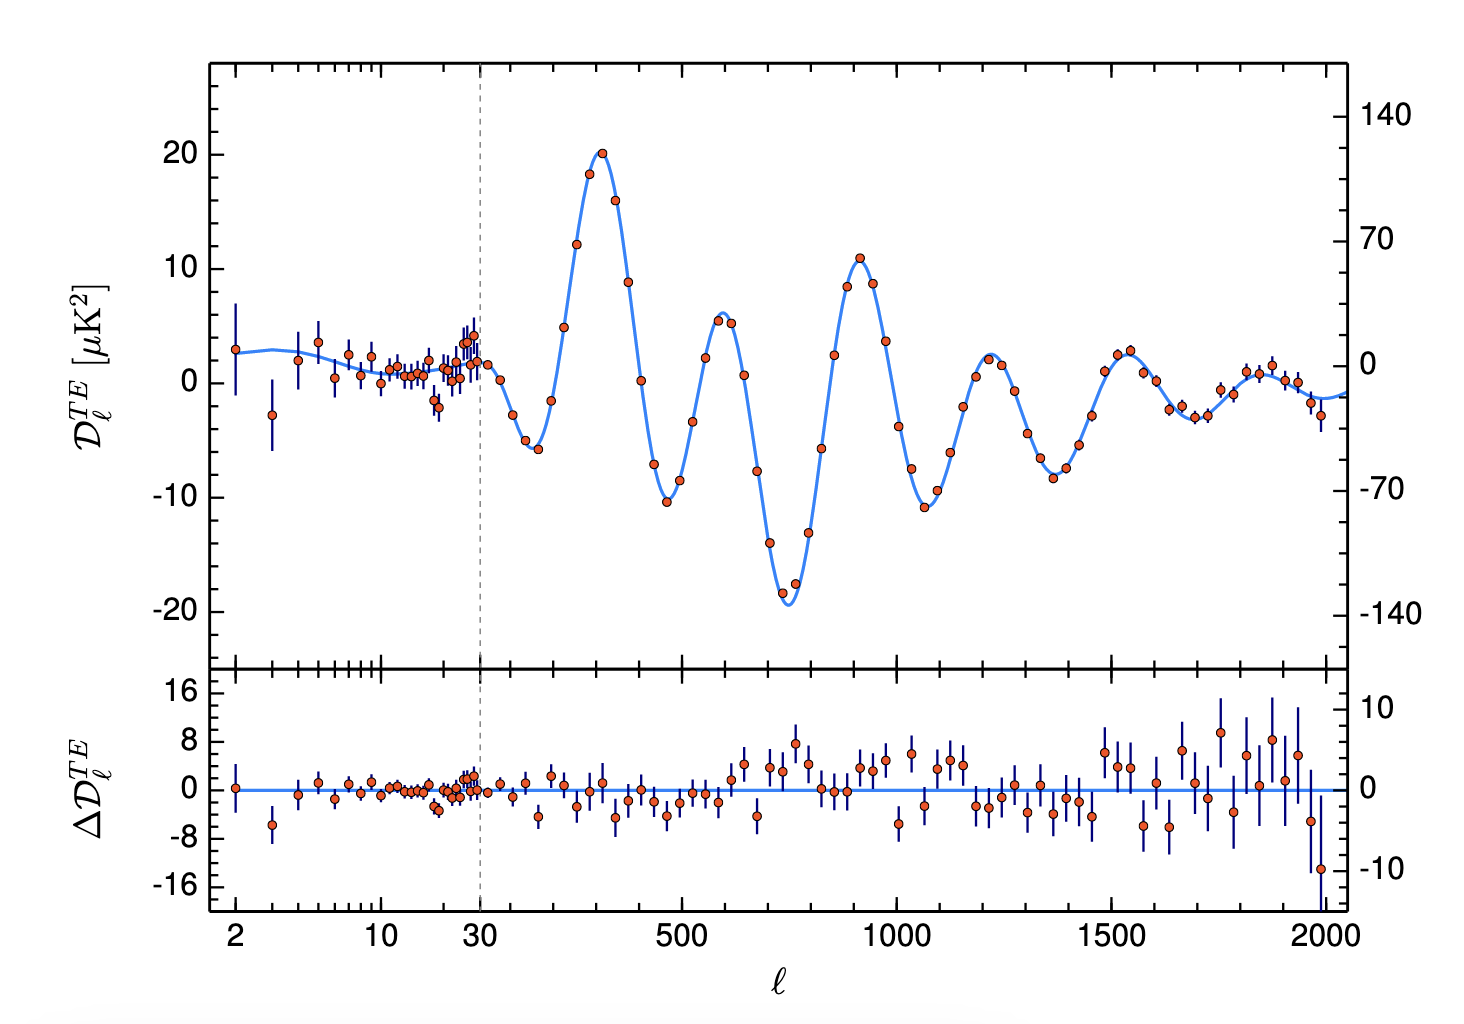
\includegraphics[width=12cm]{plots/planck_TE.png}
    \caption{Planck TE power spectrum}
    \label{fig:planck_te}
\end{figure}
\begin{figure}
    \centering
    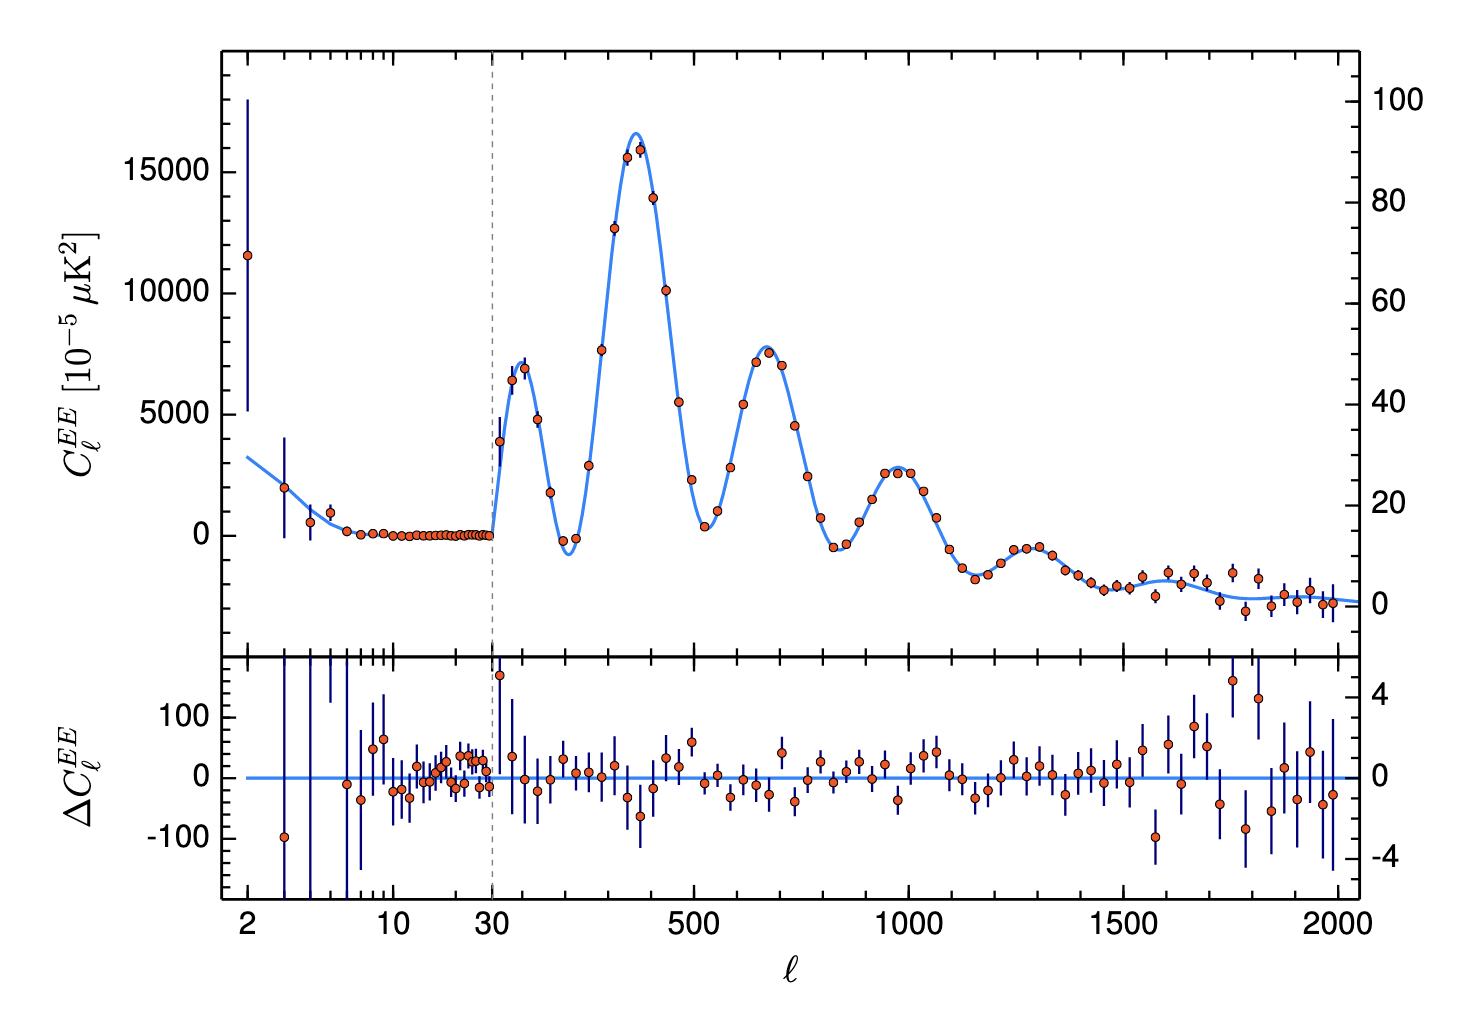
\includegraphics[width=12cm]{plots/planck_EE.png}
    \caption{Planck EE power spectrum}
    \label{fig:planck_ee}
\end{figure}
The other two power spectra are shown in figures~\ref{fig:planck_te} and~\ref{fig:planck_ee}. The main consideration with these two power spectra is to observe the way it breaks the degeneracy between $\tau_\mathrm{rei}$ and $\mathcal{A}_s,n_s$. In the TT case,  $\tau_{\mathrm{rei}}$ suppresses the power spectrum as it suppresses the fraction of light that reaches an observer. However, the additional scattering actual causes anisotropies in the polarization power spectrum to increase. Thus, the effects of $\mathcal{A}_s$ and $\tau_\mathrm{rei}$ are similar in the TT power spectrum but opposite in the $EE$ power spectrum. Thus, one needs all 3 power spectra to reliably infer the cosmological parameters.
\section{Tensions Between Weak Lensing and the CMB}
As seen, there are a total of five parameters needed to describe $\Lambda$CDM in weak lensing: $\Omega_m$, $\Omega_b$, $H_0$, $\mathcal{A}_s$, and $n_s$. This parameterization is not unique. Another common parameter, which tracks $\mathcal{A_s}$, is $\sigma_8$
\begin{equation}
	\sigma_8^2 = \left.\int\limits_0^\infty P(k,r)\left(\frac{3j_1(kr)}{kr}\right)^2\frac{k^2}{2\pi^2}dk\right|_{r=8}
\end{equation}
which can be described as the amplitude of matter fluctuations at the scale $8 h^{-1}\mathrm{Mpc}$. With this parameter instead of $\mathcal{A}_s$, weak lensing gives string constraints on $S_8 = \sigma_8\sqrt{\Omega_m/0.3}$. 

The reality is, however, that CMB measurements of some of these parameters differ between the parameters measured from weak lensing (precise results can be found in~\cite{amon_dark_2022,noauthor_planck_2018}). The most famous discrepancy is the $H_0$ tension (figure~\ref{fig:h0_tension}). Weak lensing measurements are significantly higher than CMB measurements; a nearly $5\sigma$ difference. The other famous tension is the $S_8$ tension at about a $3\sigma$ difference (figure~\ref{fig:s8_tension}). There have been extensive efforts to propose a model that can resolve these tensions (modified gravity, early dark energy, quintessence, etc.), but as of now no model can simultaneously resolve both tensions. For example, early dark energy resolves the $H_0$ tension, but the $S_8$ tension tends to either remain the same or increase. The remaining chapters will explore how to compute these tensions and demonstrate a proposed consistency test.
\begin{figure}[ht]
	\centering
	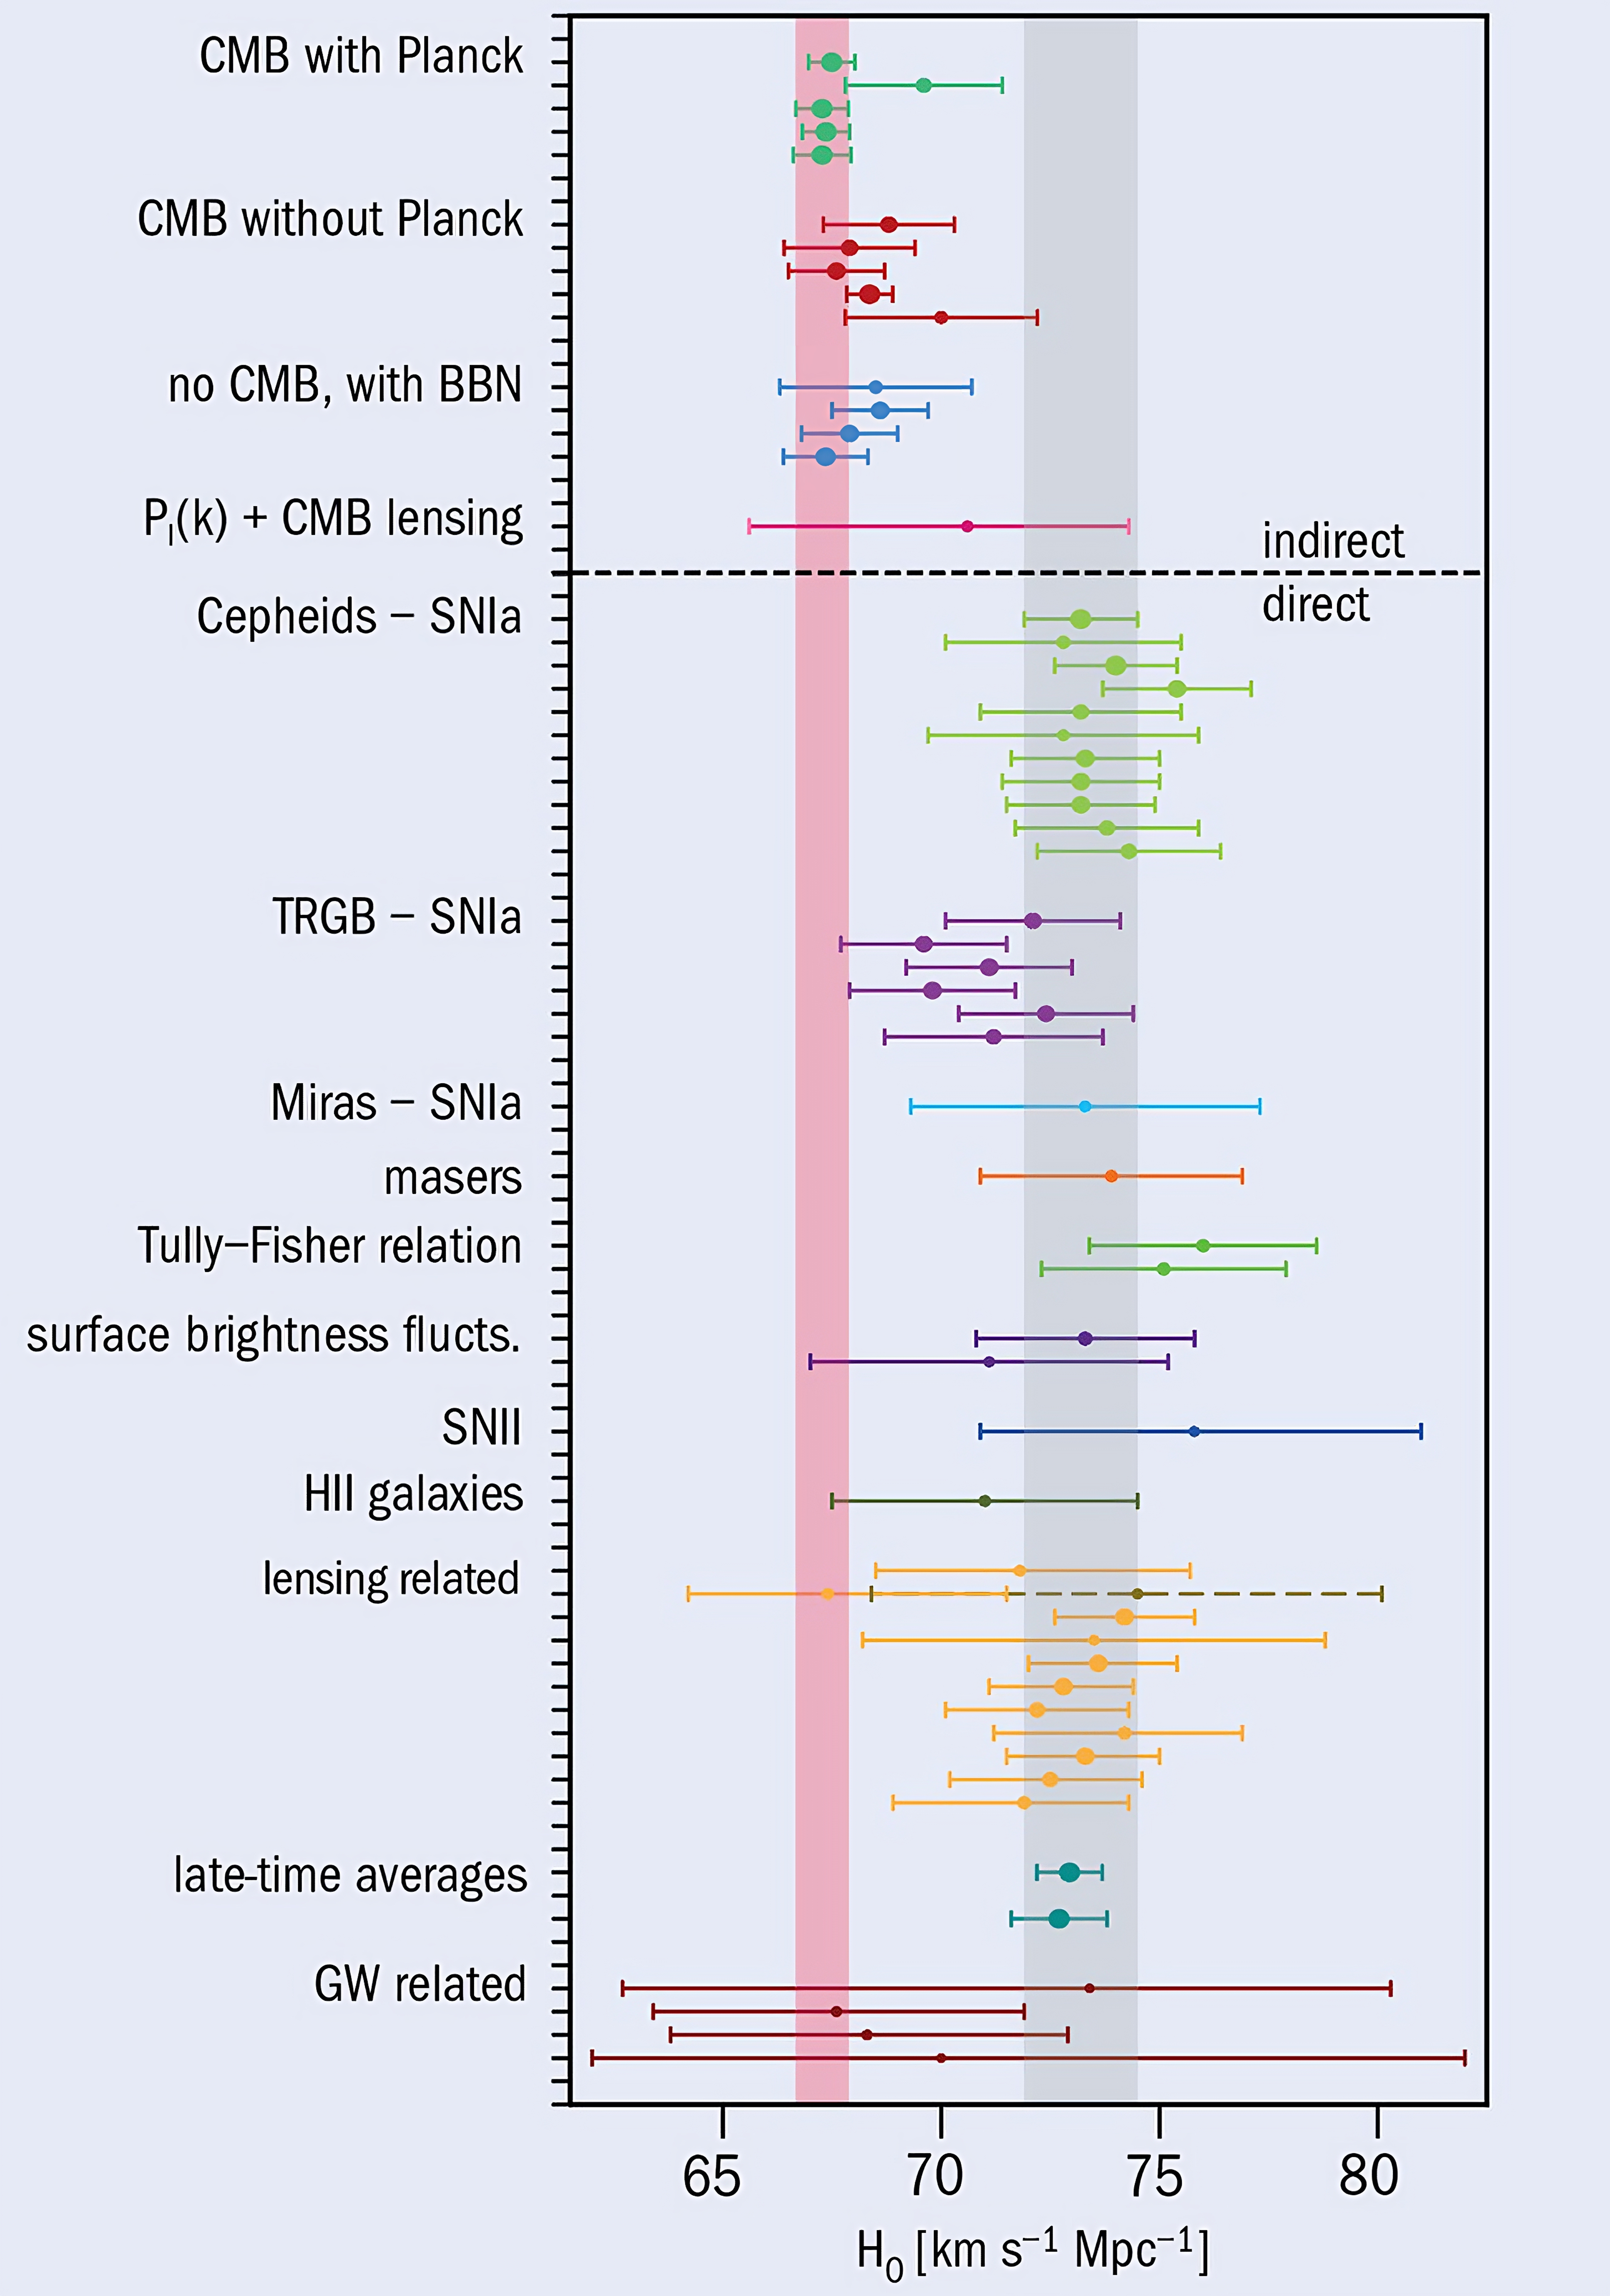
\includegraphics[width=0.75\textwidth]{plots/h0_tension_4x.jpeg}
	\caption{Measurements of $H_0$ from different experiments.}
	\label{fig:h0_tension}
\end{figure}
\begin{figure}[ht]
	\centering
	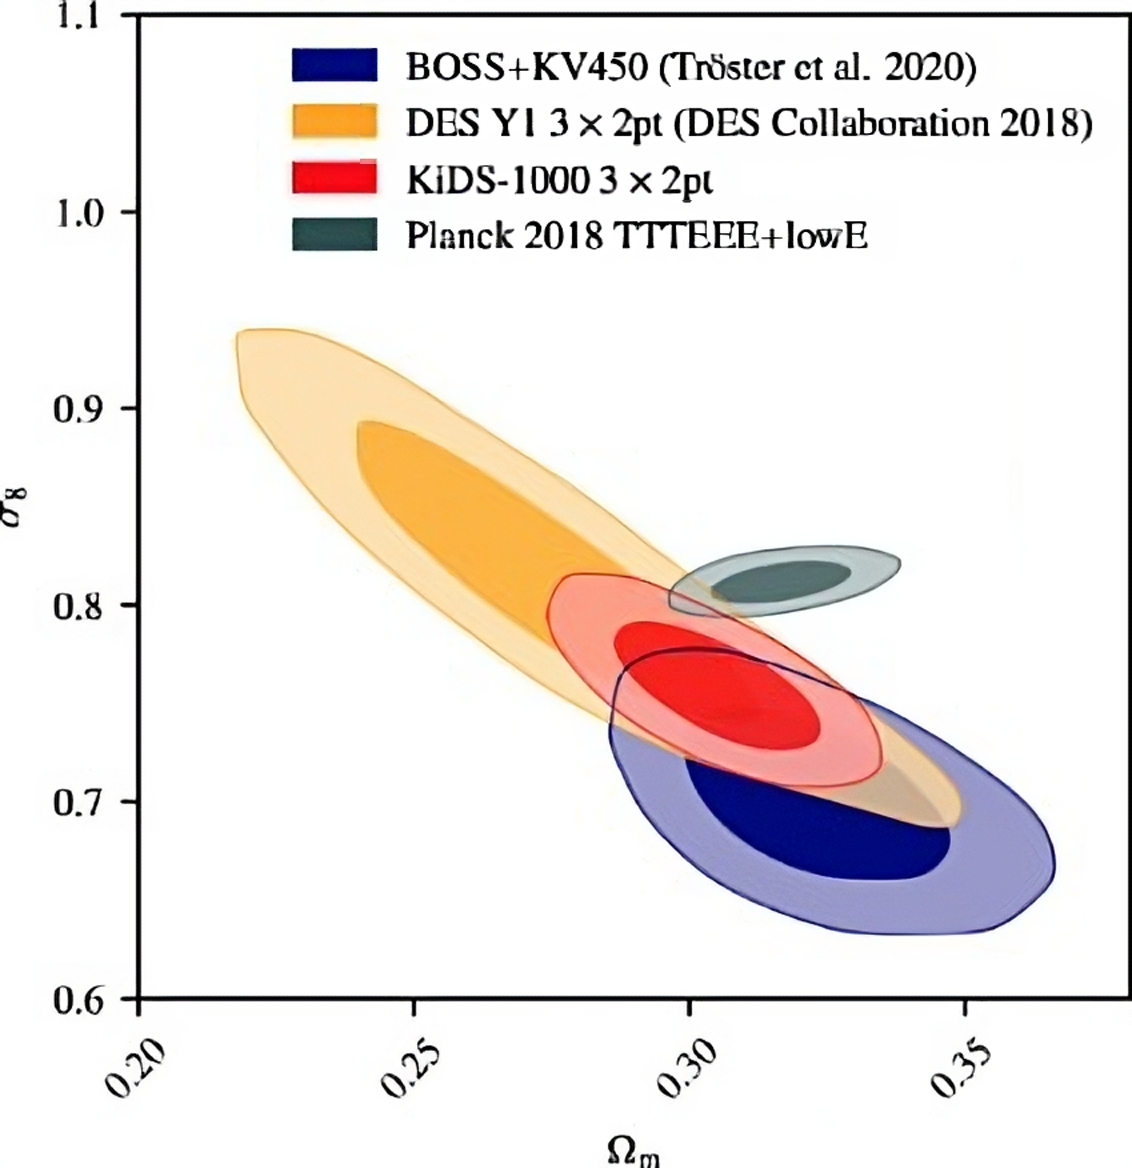
\includegraphics[width=0.75\textwidth]{plots/s8_tension_4x.jpeg}
	\caption{Measurements of $S_8$ from different experiments.}
	\label{fig:s8_tension}
\end{figure}









\chapter{Tension}
H0 and S8 tension
\section{Tension Metrics}

In a previous DES paper, the tension metrics are the following:
\begin{enumerate}
    \item Bayesian evidence ratio given by
	\[ R = \frac{\mathcal{E}_{AB}}{\mathcal{E}_A\mathcal{E}_B} \]
	Where $A$ and $B$ are data sets. This method can be written many ways using bayes theorem, which will make it appearent that this metric depends heavily on the prior volume.
    \item Bayesian suspiciousness. This metric attempts to remove the dependence on the prior volume by defining the suspiciousness as 
	\[ \log S = \log R - \log I \]
	Of particular interest here is the new value $I$ which is the information ratio, which is defined in terms of the KL divergence.
	\[ \log I = \mathcal{D}_A + \mathcal{D}_B - \mathcal{D}_{AB} \]
	\[ \mathcal{D} = \int \mathcal{P} \log(\frac{\mathcal{P}}{\Pi}) \]
    \item The method of parameter difference $\Delta$ and $n_\sigma$.
    \item Parameter difference in update form. Suppose you have two data sets $A$ and $B$. The idea is to look at the difference in mean and covariance between data set $A$ and data set $A+B$.
	\[Q_{\mathrm{UDM}} = {(\mu_A - \mu_{A+B})}^T{(C_A-C_{A+B})}^{-1}(\mu_A - \mu_{A+B}) \]
	$Q_{\mathrm{UDM}}$ will be $\chi^2$ distributed with $\rank(C_A-C_{A+B})$ degrees of freedom.
    \item Goodness of fit degredation. This is similar to the previous, where it looks at how the goodness of fit of the model in data set $A$ degrades after adding data set $B$. We have
	\[ Q_{\mathrm{DMAP}} = 2\mathcal{L}_{A}(\hat{\theta}_A) + 2\mathcal{L}_B(\hat\theta_B) - 2 \mathcal{L}_{A+B}(\hat\theta_{A+B}) \]
	with $\hat{\theta}$ being the parameter vector that maximizes the posterior, the maximum a posteriori. Again $Q_{\mathrm{DMAP}}$ is $\chi^2$ distributed. 
\end{enumerate}

\subsubsection{Metric 1: Parameter Difference}
The idea behind this metric is simple: if two data sets largely agree, there difference posterior will be centered at 0, so the integral will be close to 0.
To actually compute the integral we use the normalizing flow to learn the posterior and perform MCMC inegration. The integration error is determined using the Clopper-Pearson interval on the binomial distribution.

\subsubsection{Metric 2: Eigentension}
This metric is interesting.
We start by diagonalizing the covariance matrix on one of our data sets.
Then we take the ratio of the variance in the prior to the variance in the posterior and apply an ad hoc cut to determine which eigenmodes are well-measured.
The idea is that we should not include poorly measured eigenmodes in our tension analysis because the difference is dominated by the prior rather than the data itself.
Lastly we project the other data set onto the eigenmodes and perform the parameter difference metric on only the well-measured eigenmodes.

(here is a good place to compare with metric 1)

\subsubsection{Metric 3: Parameter Difference in Update Form}
As discussed above, we can compute the parameter $Q_{\mathrm{UDM}}$ by
\begin{equation}
    Q_{\mathrm{UDM}} = {(\mu_A - \mu_{A+B})}^T{(C_A-C_{A+B})}^{-1}(\mu_A - \mu_{A+B}) 
\end{equation}
The difference of means is precisely the mean of the parameter difference distribution, and we are using the covariance $C_A+C_{A+B}$.
Thus it is clear $Q_{\mathrm{UDM}}$ is $\chi^2$ distributed with degrees of freedom given by $\rank(C_A-C_{A+B})$. 
It is clear, however, that this metric relies on the parameter difference to be gaussian distributed because of its reliance on $Q_{\mathrm{UDM}}$ being $\chi^2$ distributed. Despite this, we proceed anyway. With proper calibration this metric can be useful even for non-gaussian posteriors.

\subsubsection{Metric 4: Goodness of Fit Degradation}

\subsubsection{Interpreting the Results}

Given some probability $P$ of a parameter shift, the following formula can give you the number of standard deviations if the probability shift comes from a gaussian distribution
\[ n_\sigma = \sqrt{2} \text{Erf}^{-1}(P) \]
I have a notebook using two unit gaussian priors separated by a distance $a$. This example can be computed analytically.
\begin{equation*}
    \begin{split}
	\mathcal{P}(\Delta \theta) &= \frac{1}{2\pi} \int\limits_{-\infty}^{\infty} e^{-\theta^2/2} e^{-{(\theta-\Delta\theta)}^2/2}  d\theta \\
				   &= \frac{1}{2\pi} \cdot \sqrt{\pi} e^{-{(\Delta\theta)}^2/4}\\
				   &= \frac{1}{\sqrt{4\pi}}e^{-{(\Delta\theta)}^2/4}\\
    \end{split}
\end{equation*}
The parameter difference posterior is a gaussian with standard deviation $\sqrt{2}$. The separation is fixed by $a$, hence the shift is $\mathcal{P}(a)$. Hence the shift probability is
\[ \Delta = \int\limits_{-a}^{a} e^{-{(\Delta\theta)}^2/4} d\Delta\theta \]
Lets use the example $a=2$. Then $n_\sigma = 2/\sqrt{2} = \sqrt{2}$. Using this we can work backwards to find $\Delta$ from a $z$-table to find $\Delta = 0.9207 - 0.0793 = 0.8414 $. 

\subsection{DES v Planck Results}
\subsection{Building from previous results}
\section{Computing techniques}
\subsection{MCMC}

Interestingly, MCMC algorithms have heavy analogies with statistical mechanics which are useful to demonstrate the concept. To examine this, lets first define what a Markov Chain is.
\begin{defn}
A sequence $X_1,\hdots,X_n$ of random elements is a \textit{Markov Chain} if the conditional distribution $X_{n+1}$ depends only on $X_n$. The set in which $X_i$ take values is called the \textit{state space} of the chain.
\end{defn}


\subsubsection{The Metropolis-Hastings Algorithm}
Suppose we want to sample from a distribution $p(x)$. $p(x)$ can be high dimensional and is generally difficult to calculate (evidence is hard to compute since it requires integration over the entire parameter space). The goal is to use Markov Chains to sample from $p(x)$ without needing to compute the evidence. This will be represented as a path through state space until the chain reaches a stable point (stationary state).

We start with a proposal distribution $g(x_n)$. Sample from the proposal distribution to find the next state $x_{n+1}$ with probability $g(x_{n+1}|x_n)$. This transition from state $n$ to state $n+1$ must follow the \textit{detailed balance condition}
\[ p(x_n) g(x_{n+1}|x_n) A(x_n \rightarrow x_{n+1}) = p(x_{n+1}) g(x_n|x_{n+1}) A(x_{n+1} \rightarrow x_{n}) \]
where $A$ is an \textit{acceptance probability} which I will define more precisely later. Using Bayes' Theorem on $p(x)$, the evidence cancels out on each side, and thus the detailed balance condition can be simplified to only rely on the likelihood and prior of $p(x)$, which I will denote $\pi$ and $\mathcal{L}$.
\[ \pi(x_n)\mathcal{L}(x_n) g(x_{n+1}|x_n) A(x_n \rightarrow x_{n+1}) = \pi(x_{n+1}) \mathcal{L}(x_{n+1}) g(x_{n}|x_{n+1}) A(x_{n+1}\rightarrow x_{n}) \]
\[ \Rightarrow \frac{A(x_n \rightarrow x_{n+1})}{A(x_{n+1}\rightarrow x_{n})} = \frac{\pi(x_{n+1}) \mathcal{L}(x_{n+1}) g(x_{n}|x_{n+1})}{\pi(x_n)\mathcal{L}(x_n) g(x_{n+1}|x_n)} \equiv R_{n,n+1} \]
This allows us to define the acceptance probability as
\[ A(x_n \rightarrow x_{n+1}) = \min( 1, R_{n,n+1} ) \]
This probability is used to determine whether the chain moves to $x_{n+1}$ or stays at $x_n$. The chain converges when it reaches a stationary state.

There are a few properties that can be observed for this algorithm:
\begin{itemize}
    \item Having an asymmetrical proposal $g(x)$ can allow for faster convergence of the chain.
    \item The initial sampling may not accurately reflect samples for $p(x)$. This is regarded as the `burn-in' and is generally discarded from the samples.
    \item MCMC Sampling loses sampling power for multi-modal distributions. 
\end{itemize}

\subsection{Data Emulators}

Traditional methods of computing likelihoods (e.g. \textsc{cosmosis}) require an immense number of CPU hours, and since we need tens of thousands of chains, we cannot rely on these traditional methods. To accelerate likelihood computation, and thus the MCMC process, we employ emulators which are neural networks that map the cosmological parameters to data vectors. The map is highly non-linear and thus a straightforward analytic mapping is not known. The neural network architecture used is similar for each experiment.

\subsubsection{LSST Emulator}
Unfourtunatly, we do not have access to the training samples for this emulator. We can however approximate the training region. First, we must define what tempered MCMC means. As discuss in the previous section, an MCMC decides wheather to accept or reject a point based on the detailed balance condition. In our case, we want to ensure the training samples cover a wide range in the parameter space, so we can modify the posterior by raising it to a power $T$ called the tempering factor. The detailed balance condition becomes

\[ \frac{A(x_n \rightarrow x_{n+1})}{A(x_{n+1}\rightarrow x_{n})} = \left[\frac{\pi(x_{n+1}) \mathcal{L}(x_{n+1})}{\pi(x_n)\mathcal{L}(x_n)}\right]^T \frac{ g(x_{n}|x_{n+1}) }{ g(x_{n+1}|x_n)} \]

It is believed the samples were generated via MCMC with a posterior tempering of $0.5$. This gives us the following distribution

\subsubsection{Planck $C_\ell$ Emulator}

Fortunately the training samples for \textsc{cosmopower} are available for download from google drive.

\subsection{Normalizing Flows}

The method of normalizing flows (MAF) implemented here uses Masked Autoencoders (MADE) to construct the flow. Suppose we have an input to the flow $x_i$. The output of the map is $y_i= \mu(x_{1:i-1})+\sigma(x_{1:i-1})x_i$. The $\mu$ and $\sigma$ are found using neural networks which recieve masked inputs $x_{1:i-1}=(x_1,\ldots,x_{i-1},0,\ldots,0)$. Since the input only depends on the first $i-1$ inputs, the normalizing flow is \textit{autoregressive} and the Jacobian is triangular.

The implementation in tensorflow uses \textit{bijectors} which implements a local diffeomorphism between a manifold $M$ and a target manifold $N$ (which are our parameter spaces), i.e. $\phi:M\rightarrow N$ such that $\phi$ is differentiable and injective. In tensorflow it has three operations, Forward, Inverse, and log\_deg\_jacobian, which are exactly the three we want. By constructing a bijector for each masked input, the full normalizing map can be constructed.

To give a motivation, I will begin with a 2 dimensional example. In this example I used \textsc{cobaya} to generate samples from two distributions. One is a pure gaussian centered at $(1/2,1/2)$ with covariance $0.005 I$  ($I$ is the identity matrix). The other is a circle of radius 1 with points generated by a gaussian based on its distance from the circle. In other words, it is a gaussian centered at $x^2+y^2$ with a mean of $x^2+y^2=1$ and a standard deviation $0.02$.

The first step is to find the parater difference distribution. Wrap the samples in the shorter chain until it is the same length as the longer chain, then take the difference of the two chains. In this example we get the following.

Now we can do the normalizing flow. As a general rule-of-thumb, the network will consist $2d$ MAfs each of $2$ hidden layers with $2d$ hidden units each, with $d$ the dimension of the distribution.
This will generally give an expressive model without introducing error from the inability to train all of the models parameters in a reasonable time. 
These parameters are tunable to whatever the user will decide, and some experimentation with these parameters is needed to ensure the best results.
In addition, we allow the parameters to be arbitrarily permuted between each MAF since the resulting probability of shift should be independent of parameterization.

One advantage of normalizing flows is its effectiveness for smaller data sets. (talk about NF vs KDE when the data is available).
\newpage
\chapter{Multifield Dark Energy}
So I don't keep having to look at this
\begin{defn}
Given a semi-riemannian manifold $M$ with metric $g$, the christoffel symbols are given by
$$ \nabla_a\partial_b = \Gamma^c_{ab}\partial_c $$
$$ \partial_ag_{bc} + \partial_bg_{ca} - \partial_cg_{ab} = 2g_{dc}\Gamma^d_{ab} $$
\end{defn}
Consider a metric of the form diag$(-1,a^2(t))$, so its determinant is $-a^6$.
The action is
$$ S=\int d^4x \sqrt{-g} \left[ \frac{1}{2}M_{p}^2 R -\frac{1}{2}\gamma_{ab}\partial_\mu\phi^a\partial^\mu\phi^b - V(\phi)+\mathcal{L}_m \right] $$
I only want to describe a homogeneous background, so the field is only a function of time. The action becomes
$$ S=\int d^4x \sqrt{-g} \left[ \frac{1}{2}M_{p}^2 R -\frac{1}{2}\gamma_{ab}\dot\phi^a\dot\phi^b - V(\phi)+\mathcal{L}_m \right] $$
Varying the field gives
$$ \delta S = \int d^4x \sqrt{-g}\left[ - \frac{1}{2}\partial_a(\gamma_{bc})\dot\phi^b\dot\phi^c - \frac{1}{2}\gamma_{ab}\frac{d}{dt}(\delta\phi^a)\dot\phi^b - \partial_aV\delta\phi^a \right] $$
$$ \delta S = -\frac{1}{2}(\delta\phi^a)(\sqrt{-g}\gamma_{ab}\dot\phi^b + \int d^4x \sqrt{-g}\left[ -\frac{1}{2}\gamma(\nabla_a\partial_b,\partial_c)\dot\phi^b,\dot\phi^c -\frac{1}{2}\gamma(\partial_b,\nabla_a\partial_c)\dot\phi^b\dot\phi^c + 3\frac{\dot a}{a}\gamma_{ab}\delta\phi^a\dot\phi^b + \gamma_{ab}\delta\phi^a\ddot\phi^b -V_a\delta\phi^a \right] $$
$$ \delta S = -\int d^4x \sqrt{-g}\left[ \frac{1}{2}\Gamma_{ab}^d\gamma_{dc}\dot\phi^b\dot\phi^c + \frac{1}{2}\Gamma_{ac}^d\gamma_{bd}\dot\phi^b\dot\phi^c + 3H\gamma_{ab}\dot\phi^b + \gamma_{ab}\ddot\phi^b + V_a  \right] $$
Multiply everything by $\gamma^{aa}$. Now lets do some reshuffling of the indices.
$$ \gamma^{aa}\Gamma^d_{ab}\gamma_{dc}\dot\phi^b\dot\phi^c $$
$$ a\leftrightarrow d$$
$$ \gamma^{ad}\Gamma^a_{db}\gamma_{ac}\dot\phi^b\dot\phi^c $$
$$ b\leftrightarrow d$$
$$ \gamma^{ad}\Gamma^a_{bd}\gamma_{ac}\dot\phi^b\dot\phi^c $$
$$ \gamma^{ab}\Gamma^a_{bd}\gamma_{ac}\dot\phi^d\dot\phi^c $$
$$ c\leftrightarrow d$$
$$ \gamma^{ab}\Gamma^a_{bc}\gamma_{ad}\dot\phi^d\dot\phi^c = \Gamma_{bc}^a \dot\phi^b\dot\phi^c $$
and
$$ \gamma^{aa} \Gamma^d_{ac}\gamma_{bd}\dot\phi^b\dot\phi^c $$
$$ a\leftrightarrow d$$
$$ \gamma^{ad} \Gamma^a_{dc}\gamma_{ba}\dot\phi^b\dot\phi^c $$
$$ b\leftrightarrow d$$
$$ \gamma^{ab} \Gamma^a_{bc}\gamma_{da}\dot\phi^d\dot\phi^c = \Gamma_{bc}^a\dot\phi^b\dot\phi^c $$
Thus the equation of motion is found,
$$ \ddot\phi^a + \Gamma_{bc}^a\dot\phi^b\dot\phi^c +3H\dot\phi^a + V^a = 0 $$
$$ D_t\dot\phi^a+3H\dot\phi^a + V^a = 0 $$

The riemann curvature is
$$ R^\alpha_{\beta\gamma\delta} = \partial_\beta\Gamma^\alpha_{\gamma\delta} - \partial_\gamma\Gamma^\alpha_{\beta\delta}+\Gamma^\sigma_{\gamma\delta}\Gamma^\alpha_{\beta\sigma} - \Gamma^\sigma_{\beta\delta}\Gamma^\alpha_{\gamma\sigma} $$
So the Ricci curvature tensor is
$$ R_{\beta\delta} = R^\alpha_{\beta\alpha\delta} = \partial_\beta\Gamma^\alpha_{\alpha\delta} - \partial_\alpha\Gamma^\alpha_{\beta\delta}+\Gamma^\sigma_{\alpha\delta}\Gamma^\alpha_{\beta\sigma} - \Gamma^\sigma_{\beta\delta}\Gamma^\alpha_{\alpha\sigma} $$
And the Ricci scalar curvature is
$$ R = R_{\beta}^{\beta} = g^{\beta\delta}R_{\beta\delta} =
g^{\beta\delta}\partial_\beta\Gamma^\alpha_{\alpha\delta} -
g^{\beta\delta}\partial_\alpha\Gamma^\alpha_{\beta\delta}
+g^{\beta\delta}\Gamma^\sigma_{\alpha\delta}\Gamma^\alpha_{\beta\sigma} -
g^{\beta\delta}\Gamma^\sigma_{\beta\delta}\Gamma^\alpha_{\alpha\sigma} $$
Since the fields only depend on time, we only need to consider the temporal component of the Ricci curvature tensor, so
$$ R_{tt} = \partial_t \Gamma^{\alpha}_{\alpha t} - \partial_\alpha\Gamma^{\alpha}_{tt}
+ \Gamma^{\sigma}_{\alpha t}\Gamma^{\alpha}_{t \sigma} - \Gamma^{\sigma}_{tt}\Gamma^{\alpha}_{\alpha\sigma} $$
From the definition of the christoffel symbols, and noting $ g = g(t)$ and $g$ is diagonal, we have $\partial_t g_{aa} = 2g_{ba}\Gamma^b_{ta}$, thus
the second term is necessarily 0 since $\partial_t g_{tt} = 0$. The first term is non-zero for $\alpha = 1,2,3$, in which it equals 
$$ \frac{1}{2}\partial_t (1/a^2 \partial_t a^2) = \partial_t(\dot a / a) = -3\ddot a /a + 3\dot a^2 /a^2 $$
The third term is non-zero for $\alpha = \sigma$, In which case we get 
$$ \frac{3}{4a^4}(\partial_t (a^2))^2 =  -3\dot a^2/a^2  $$
The last term is vanishes since the temporal component of the metric is constant. Thus we find
$$ R_{tt} = 3\frac{\ddot a}{a}$$
Now, if we consider spatial components of the Ricci curvature, we find that the first term now vanishes, the second term is equal to $ -\ddot a/a - \dot a^2/a^2$, the thrid term is 0, and the last term is $-\dot a^2/a^2$, so the spacial components are
$$ R_{xx} = -\ddot a  a - 2\dot a^2$$
Thus the Ricci curvature scalar is
$$ 6\ddot a/a + 6\dot a^2/a^2 $$
Hence the einstein equation gives
$$ -3H^2 =  $$
I need to write out the indices better if I want to get the signs correct.

\hrule
$$ \partial_ag_{bc} + \partial_bg_{ca} - \partial_cg_{ab} = 2g_{dc}\Gamma^d_{ab} $$

\hrule
Considering the way this acts on the coordinate vector field $\partial_\alpha$, 
$$ R\partial_\alpha =
g^{\beta\delta}\partial_\beta\Gamma^\alpha_{\alpha\delta}\partial_\alpha -
g^{\beta\delta}\partial_\alpha\Gamma^\alpha_{\beta\delta}\partial_\alpha
+g^{\beta\delta}\Gamma^\sigma_{\alpha\delta}\Gamma^\alpha_{\beta\sigma}\partial_\alpha -
g^{\beta\delta}\Gamma^\sigma_{\beta\delta}\Gamma^\alpha_{\alpha\sigma} \partial_\alpha $$
$$ R\partial_\alpha =
g^{\beta\delta}\partial_\beta \nabla_\alpha\partial_\delta -
g^{\beta\delta}\partial_\alpha \nabla_\beta\partial_\delta
+g^{\beta\delta}\Gamma^\sigma_{\alpha\delta} \nabla_\beta\partial_\sigma -
g^{\beta\delta}\Gamma^\sigma_{\beta\delta} \nabla_\alpha \partial_\sigma $$


%\section{Perturbat{}ion Theory}
%\input{perturb{}ation.tex}

%\section{Computing}
%\input{computing.tex}

%\section{Fields}
%\input{field.tex}

\end{document}
